%!TEX root = ../terrainbook.tex

\graphicspath{{bathymetry/}}

\chapter{Processing bathymetric data to produce hydrographic charts}
\label{chap:bathymetry}

\begin{figure}[h]
  \centering
  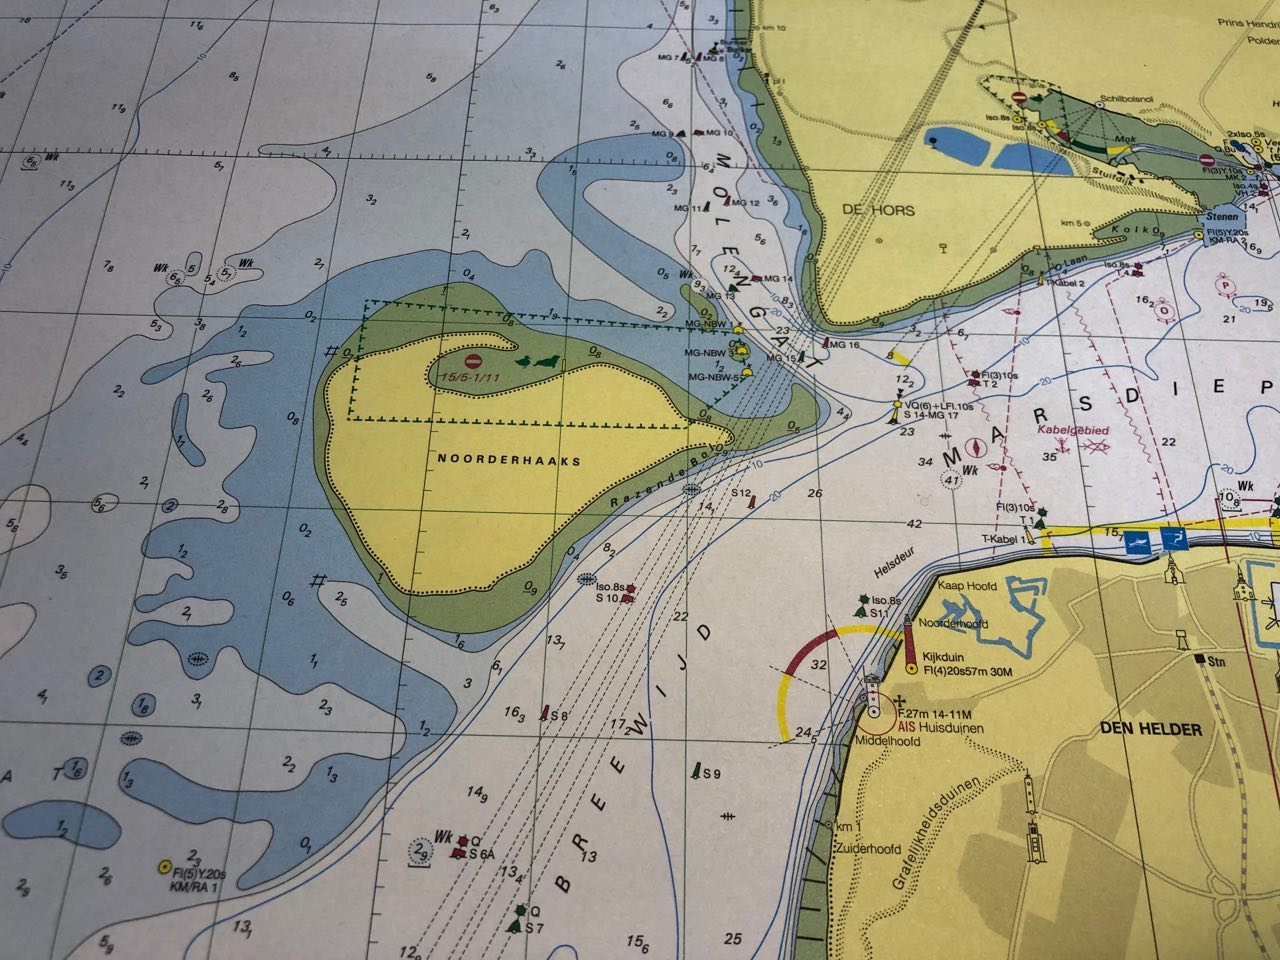
\includegraphics[width=0.8\linewidth]{figs/enc_denhelder.jpeg}
  \caption{An example of an ENC (electronic navigational chart) in the Netherlands. [photo of a paper map from the \emph{Hydrografische Dienst}]}
\label{fig:enc.jpg}
\end{figure}

An hydrographic chart is a map of the underwater world specifically intended for the safe navigation of ships.
In its digital form, it is often called an electronic navigational chart, or ENC.
The information appearing on an ENC are standardised, and there are open formats.

%

We focus in this chapter on one element of these charts: depth-contours.
These are contour lines that, instead of elevation, show the depth with respect to a given level of water.
The creation of these depth-contours from an input point cloud of depth measurements requires many tools that were introduced in this book; Delaunay triangulation and the Voronoi diagram (Chapter~\ref{chap:dtvd}), interpolation (Chapter~\ref{chap:interpol}), and contour generation from a TIN (Chapter~\ref{chap:conversion}).


%%%
%
\section{How are depth-contours produced in practice?}

Traditionally, depth-contours were drawn by hand by skilled hydrographers.
They used a sparse set of scattered surveyed depth measurements to deduct and depict the morphology of the seafloor with smooth-looking curves.

%

Nowadays, with technologies such as multibeam echosounders (MBES) offering an almost full coverage of the seafloor (see Section~\ref{sec:mbes}), one would expect the contouring process to be fully automatic.
It is however in practice still a (semi-)manual process since the new technologies have ironically brought new problems: computers have problems processing the massive amount of data, especially in choosing which data is relevant and which is not.
%It also turns out to be challenging to guarantee that the contours are both pleasing to read and safe.

%

The raw contours constructed directly from MBES datasets are often not satisfactory for navigational purposes since, as Figure~\ref{fig:raw} shows,
\begin{figure}
  \centering
  \begin{subfigure}[b]{0.45\linewidth}
    \centering
    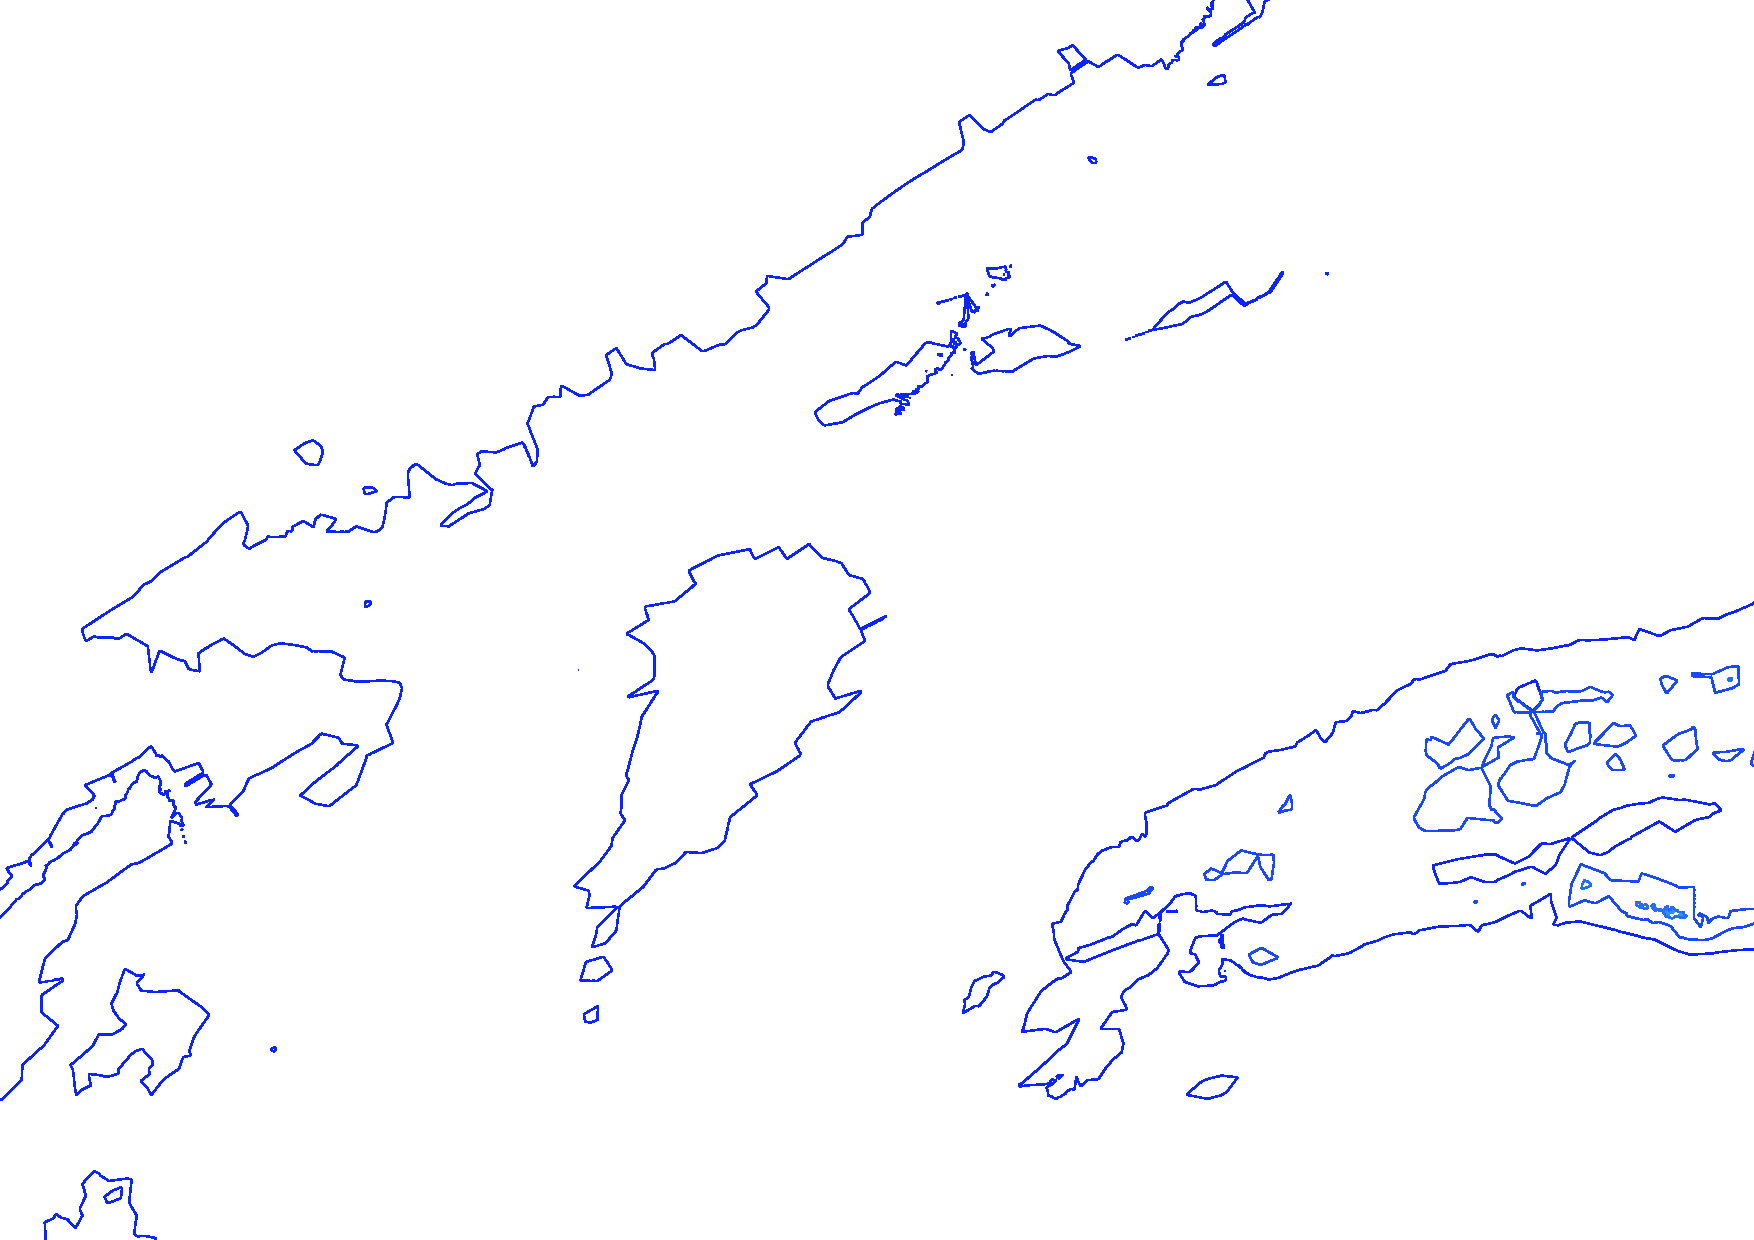
\includegraphics[width=\textwidth]{figs/raw.pdf}
    \caption{}\label{fig:raw}
  \end{subfigure}%
  \begin{subfigure}[b]{0.45\linewidth}
    \centering
    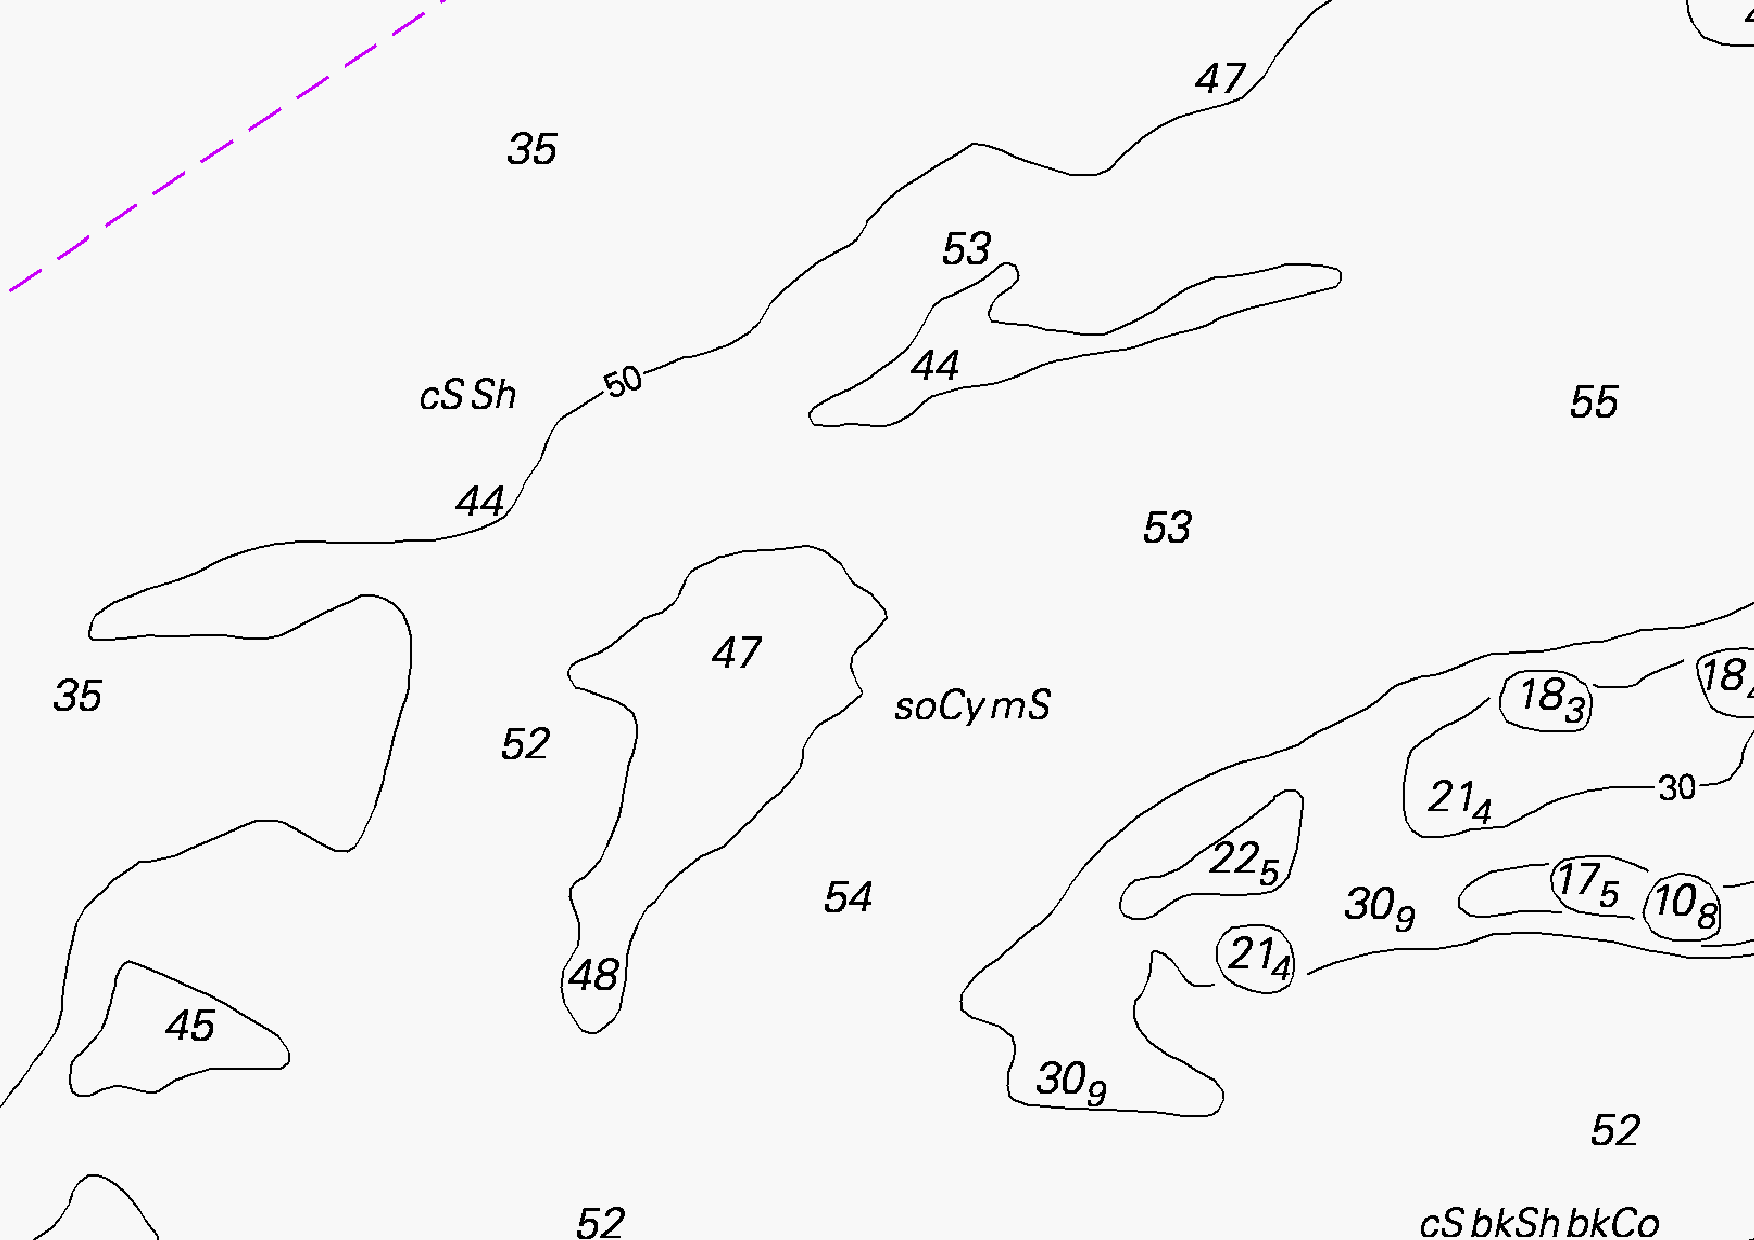
\includegraphics[width=\textwidth]{figs/maponly.pdf}
    \caption{}\label{fig:ideal}
  \end{subfigure}
  \begin{subfigure}[b]{0.45\linewidth}
    \centering
    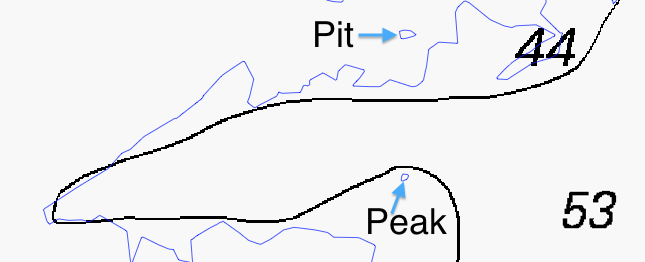
\includegraphics[width=\textwidth]{figs/smoothinAndOmission.png}
    \caption{}
  \end{subfigure}
  \begin{subfigure}[b]{0.45\linewidth}
    \centering
    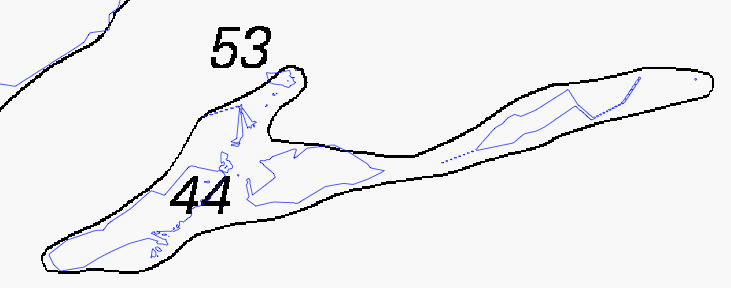
\includegraphics[width=\textwidth]{figs/aggregation.png}
    \caption{}\label{fig:aggregation}
  \end{subfigure}
\caption{Comparison of \textbf{(a)} depth-contours obtained automatically from the raw MBES data and \textbf{(b)} the hydrographic chart from the Royal Australian Navy for the Torres Strait north of Australia. Raw depth contours are blue, generalized depth contours are black. \textbf{(c)} Pits are removed, while peaks are preserved or integrated with another contour. \textbf{(d)} Groups of nearby contour lines are aggregated}
\label{fig:contouringaspects}
\end{figure}
they are zigzagging (the representation of the seafloor thus contains ``waves'', \ie\ the slope changes abruptly) and they contain many ``island'' contours (seafloor has several local minima and maxima). 
These artefacts are the result of measurement noise that is present in MBES datasets, \ie\ the variation in depth between two close samples can be larger than in reality, even after the dataset has been (statistically) cleaned.
Figure~\ref{fig:ideal} illustrates what is expected by hydrographers.


%%%%%%%%%%%%%%%%%%%%
%
\subsection{Generalisation is required to obtain good depth contours}
\label{sec:good-depth-contours}

Creating good depth-contours requires \emph{generalisation}, \ie\ the process of meaningfully reducing information.

%

The process of generalisation is guided by constraints that essentially define when a depth-contour is ``good''.
A good depth contour satisfies all of the following four generalisation constraints.
\begin{enumerate}
  \item The \emph{safety constraint}.  
  At every location, the indicated depth must not be deeper than the depth that was originally measured at that location; this is to guarantee that a ship never runs aground because of a faulty map.
  This constraint is a so-called hard constraint, \ie\ it can never be broken.
  \item The \emph{legibility constraint}. 
  An overdose of information slows down the map reading process for the mariner, thus only the essential information should be depicted on the map in a form that is clearly and efficiently apprehensible. %This requires cartographic generalisation.
  \item The \emph{topology constraint}. 
  The topology of the depicted map elements must be correct, \ie\ isocontours may not touch or intersect (also a hard constraint).
  \item The \emph{morphology constraint}. 
  The map should be as realistic and accurate as possible, \ie\ the overall shape of the morphology of the underwater surface should be clearly perceivable and defined features should be preserved.
\end{enumerate}

It should be noted that these four constraints are sometimes incompatible with each other. 
For instance, the morphology constraint tells us to stay close to the measured shape of the seafloor, while the legibility constraint forces us to deviate from that exact shape by disregarding details. 

%

Also, because of the safety constraint, depth-contours can only be modified such that the safety is respected at all times: contours can only be pushed towards the deeper side during generalisation, as illustrated in Fig~\ref{fig:genvalidornot}. 
\begin{figure}
  \centering
  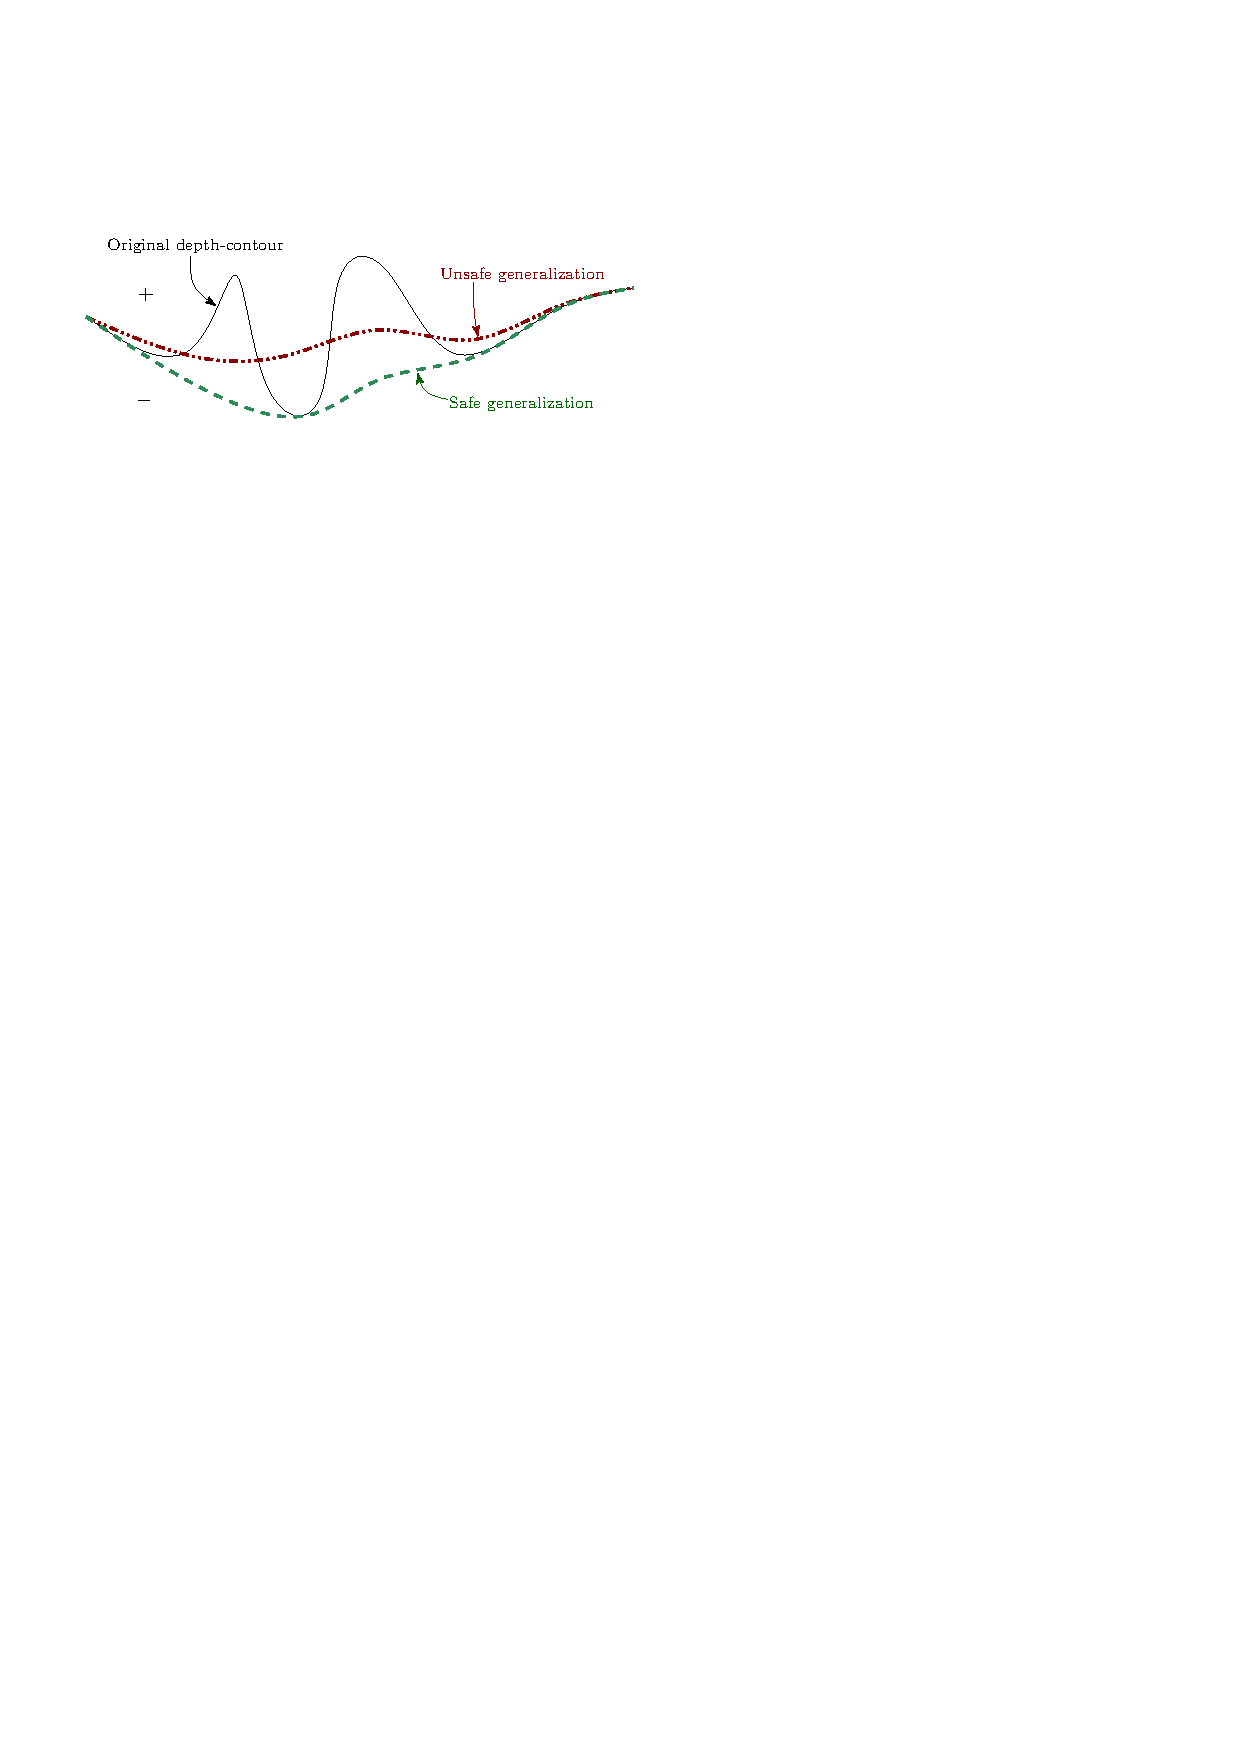
\includegraphics[width=0.5\textwidth]{figs/genvalidornot}
  \caption{During generalisation, depth-contours can only be moved towards greater depth (indicated by a ``--'' in the figure).}
\label{fig:genvalidornot}
\end{figure}
It is therefore obvious that the end result must be a reasonable compromise between the four constraints, although the hard constraints must not be broken.


%%%
\section{Common methods used in practice are not satisfactory}

The generation of depth contours, and their generalisation, can be done by several methods.
We present here the most frequently used methodologies to generate depth-contours from an MBES point cloud.

% We demonstrate in the next section that such workflows can \emph{not} guarantee that the safety constraint is respected, and should therefore not be used.

%%%
\subsection{Displacement and generalisation of the lines}

It is tempting to start with the raw contours lines and use a generalisation operator to simplify them, \eg\ the Douglas-Peucker method.
It should however be noticed that this method does \emph{not} guarantee that the safety constraint will be respected, that is the generalised line will be ``pushed'' both to the deeper and the shallower part (there is no control for this with the Douglas-Peucker method).

There exist a few algorithms to control the direction in which a line can be moved (these methods are outside the scope of this book), but these methods work only on lines individually and thus the resulting set of lines can contain intersecting lines.
Furthermore, this solution does not solve the presence of many island contours, or can at best delete the small ones (and not aggregate them as in Figure~\ref{fig:aggregation}).

%%%
\subsection{Creation of a simplified raster}

Practitioners usually first interpolate the original MBES samples to create a (coarse) grid and then directly extract the contours from the grid.
If the number of samples is too high to be processed by a computer, they often use a subset, which has the added benefits of creating smoother and simpler depth-contours.

%

The following are methods that use a raster data structure either to select a subset of the input samples or to construct a raster surface.


%
\paragraph{Selection with virtual gridding.}
This is a point filtering method that aims at reducing the volume of data, in order to create generalised contours and to speed up the computation time, or simply to make the computation possible, in the case the input dataset is several orders of magnitude bigger than the main memory of a computer.
The idea is to overlay a virtual grid on the input points and to keep one point for every grid cell.
The selected points can either be used to construct a raster or TIN surface, see below.
While different functions can be used to select the point (\eg\ deepest, shallowest, average, or median), because of the safety constraint the shallowest point is often chosen by practitioners, see Figure~\ref{fig:fr:vg:a} for a one-dimensional equivalent.
\begin{figure}
\centering
  \begin{subfigure}[b]{0.3\linewidth}
    \centering
    \includegraphics[width=\textwidth,page=2]{figs/virtualgridding.pdf}
    \caption{Virtual gridding}\label{fig:fr:vg:a}
  \end{subfigure}
  \qquad
  \begin{subfigure}[b]{0.3\linewidth}
    \centering
    \includegraphics[width=\textwidth,page=2]{figs/maxgridding.pdf}
    \caption{Max rasterisation}\label{fig:fr:mg:a}
  \end{subfigure}
  \qquad
  \begin{subfigure}[b]{0.3\linewidth}
    \centering
    \includegraphics[width=\textwidth,page=4]{figs/1Didw.pdf}
    \caption{IDW rasterisation}\label{fig:fr:idw:a}
  \end{subfigure}
  \qquad
  \quad
  \begin{subfigure}[b]{0.3\linewidth}
    \centering
    \includegraphics[width=\textwidth,page=3]{figs/virtualgridding.pdf}
    \caption{Virtual gridding and TIN-based contour values}\label{fig:fr:vg:b}
  \end{subfigure}
  \qquad
  \begin{subfigure}[b]{0.3\linewidth}
    \centering
    \includegraphics[width=\textwidth,page=3]{figs/maxgridding.pdf}
    \caption{Max rasterisation and contours}\label{fig:fr:mg:b}
  \end{subfigure}
  \qquad
  \begin{subfigure}[b]{0.3\linewidth}
    \centering
    \includegraphics[width=\textwidth,page=5]{figs/1Didw.pdf}
    \caption{IDW rasterisation and contours}\label{fig:fr:idw:b}
  \end{subfigure}
\caption{On the top: profile views of different filtering and rasterisation methods. On the bottom: the corresponding contours. The arrows indicate where the safety constraint is violated with respect to the original points. Also note that in case a grid cell contains no data, no contours can be derived.}
\label{fig:filterraster}
\end{figure}
It should however be stressed that choosing the shallowest point does not guarantee safe contours. 
The problem is that contour extraction algorithms perform a linear interpolation on the raster cells. 
As can be observed from Figure~\ref{fig:fr:vg:b}, this easily results in safety violations at `secondary' local maxima in a grid cell. 
The number and severity of these violation is related to the cellsize of the virtual grid: a bigger cellsize will result in more and more severely violated points.
Notice that it is not possible to reduce the cellsize such that the safety issue can be guaranteed.  

%
\paragraph{Max rasterisation.}
As Figure~\ref{fig:fr:mg:a} shows, it is similar to virtual gridding, the main difference is that a raster (a surface) is created where every cell in the virtual grid becomes a raster cell whose depth is the shallowest of all the samples.
This disregards the exact location of the original sample points, and moves the shallowest point in the grid cell to the centre of the pixel. 
That means that the morphology constraint is not respected.
Moreover, as Figure~\ref{fig:fr:mg:b} shows, the safety constraint is not guaranteed, for the same reasons as with virtual gridding.
Again, the severity of these problems depends on the chosen cellsize.

%
\paragraph{Interpolation to a raster.}
For hydrographic charts, the raster surface is often constructed with spatial interpolation, particularly with the method of \emph{inverse distance weighting} (IDW).
Figures~\ref{fig:fr:idw:a} and~\ref{fig:fr:idw:b} illustrate the process of IDW interpolation, notice that as a result of the averaging that takes place extrema are disregarded and subsequently the safety constraint is also violated. 

%
%\paragraph{Raster coarsening.}
%Raster coarsening is somewhat similar to max rasterisation, the difference is that it takes a raster as input rather than sample points. 
%Based on that input raster, a new raster is created that has larger cellsize. 
%In this way small details in the surface are omitted. Subsequently the contour lines that correspond to this coarsened raster surface also contain fewer small details. 
%In terms of safety this method has the same drawbacks as max rasterisation.



%%%
\subsection{TIN simplification}
  
One could use TIN simplification as explained in Chapter~\ref{chap:conversion} to simplify the riverbed.
This would also simplify the depth-contours that are generated from the TIN. 
However, as Figure~\ref{fig:simpfail} shows, 
\begin{figure}
\centering
  \begin{subfigure}[b]{0.2\linewidth}
    \centering
    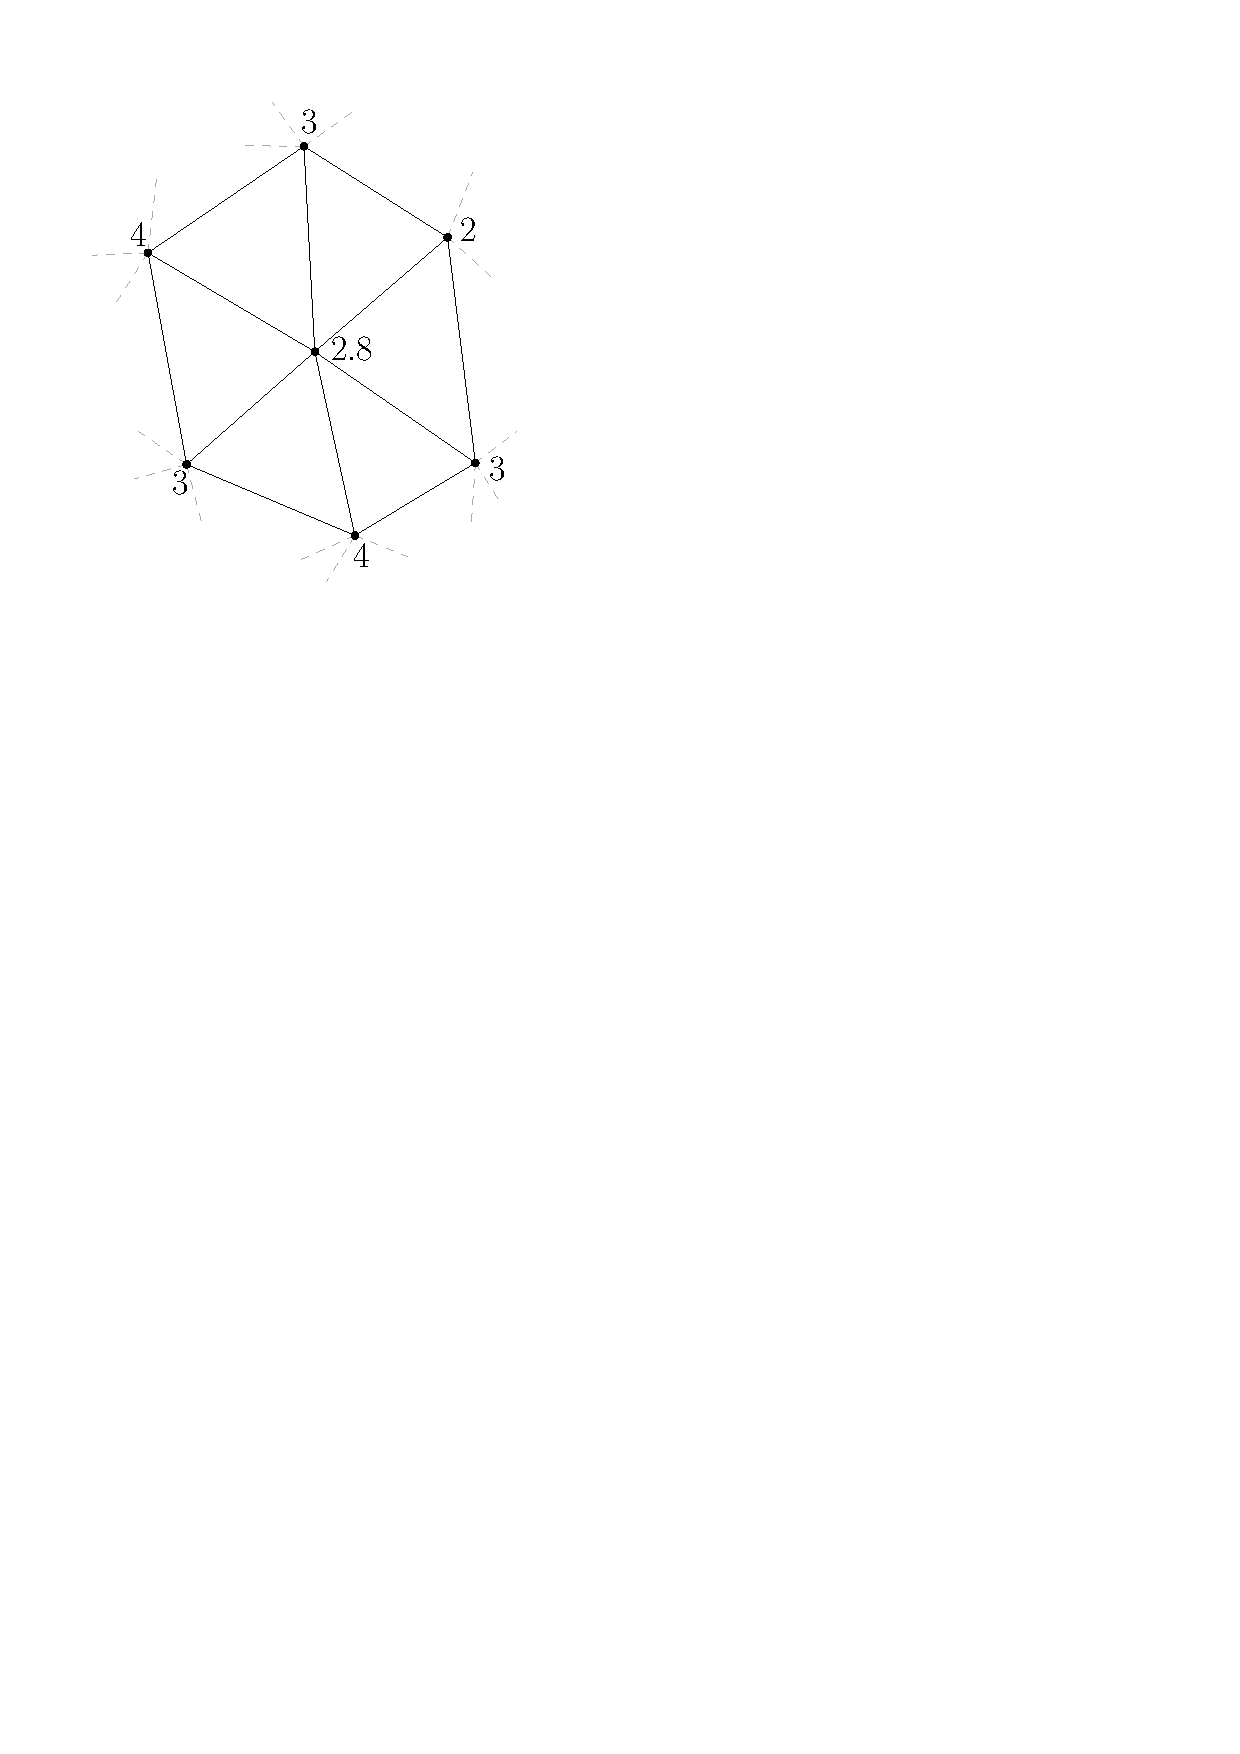
\includegraphics[width=\textwidth,page=1]{figs/simpfail.pdf}
    \caption{Initial configuration}\label{fig:simpfail:a}
  \end{subfigure}
  \qquad
  \begin{subfigure}[b]{0.2\linewidth}
    \centering
    \includegraphics[width=\textwidth,page=2]{figs/simpfail.pdf}
    \caption{1st vertex removal}\label{fig:simpfail:b}
  \end{subfigure}
  \qquad
  \begin{subfigure}[b]{0.2\linewidth}
    \centering
    \includegraphics[width=\textwidth,page=3]{figs/simpfail.pdf}
    \caption{2nd vertex removal}\label{fig:simpfail:c}
  \end{subfigure}
\caption{Due to the re-triangulation after a removal, violations of the safety constraint may occur after a series of points are removed. The first vertex is removed (locally the resulting surface will be shallower). However, the second removal changes the configuration of triangles and at that location the surface is now deeper. A lower number means a shallower point.}
\label{fig:simpfail}
\end{figure}
the safety constraint is not guaranteed to be respected when vertices are removed from a TIN.
This is due to the fact that the triangulation must be updated (with flips, see Chapter~\ref{chap:dtvd}) and the shape of the triangles are not controlled by the depth of the vertices, but rather by the Delaunay criterion.


%%%
%
\section{A Voronoi-based surface approach}

Part of the problems with existing approaches to generate depth-contours is the fact that the different processes, such as spatial interpolation, generalisation and contouring, are treated as independent processes.
These are in fact interrelated, and we introduce in the following a method where the different processes are integrated.
This method uses several of the algorithms and data structures studied in this book, and with small extensions and modifications we can obtain depth-contours that are safe and legible.

%

The key idea behind the method, called the Voronoi-based surface approach, is to have one single consistent representation of the seafloor from which contours can be generated on-the-fly (potentially for different map scales, or with varying degrees of generalisation).
Instead of performing generalisation by moving lines or using a subset of the original samples, we include all MBES points in a triangulation (the surface) and manipulate this triangulation directly with generalisation operators that fulfil the constraints listed in Section~\ref{sec:good-depth-contours}.

%

Figure~\ref{fig:surfapproach} gives a schematic overview of the different components of our Voronoi-based surface concept. 
\begin{figure}
  \centering
  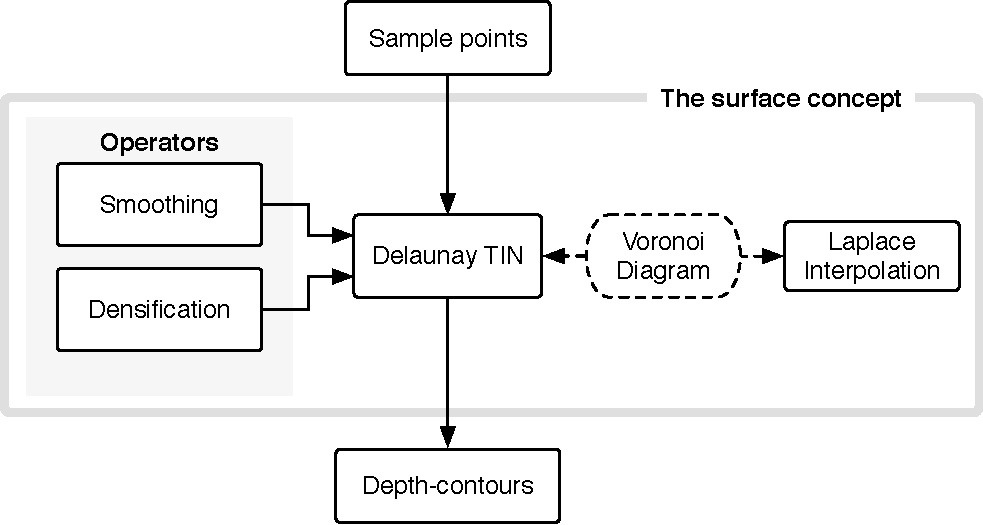
\includegraphics[width=0.7\textwidth]{figs/surfaceapproach_V2.pdf}
  \caption{Overview of the Voronoi- and surface-based approach.}
\label{fig:surfapproach}
\end{figure}

Firstly, all the input points of a given area are used to construct a Delaunay TIN.
Secondly, a number of generalisation operators are used that alter the TIN using Laplace interpolation, which is based on the Voronoi diagram.
These operators aim at improving the slope of the surface, and permit us to generalise the surface.
Finally, contour lines are derived from the altered TIN using linear interpolation.


Representing a field in a computer is problematic since computers are discrete machines.
We therefore need to \emph{discretise} the field, \ie\ partition it into several pieces that cover the whole area (usually either grid cells or triangles).
Contours in Figure~\ref{fig:raw} are not smooth basically because the seabed is represented simply with a TIN of the original samples, which is a C$^0$ interpolant.
However, as we demonstrate below, we can obtain a smooth looking approximation of the field by densifying the TIN using the Laplace interpolant (see Section~\ref{sec:laplace}), which is C$^1$.

%

Two generalisation operators allow us to obtain a smoother surface from which depth-contours can be extracted: (1) smoothing; (2) densification.


%%%
%
\subsubsection{The smoothing operator}
\label{chap:myapproach:smoothing}

The smoothing operator basically estimates, with the Laplace interpolant (see Section~\ref{sec:laplace} on page~\pageref{sec:laplace}), the depth of each vertex in a dataset by considering its natural neighbour (see Figure~\ref{fig:1Dsmoothop}).
If this depth is shallower, then the vertex is assigned this value; if it is deeper than nothing is done.
Thus, the smoothing operator does not change the planimetric coordinates of vertices, but only lifts the vertices' depths. 
\begin{figure}[tbh]
  \centering
  \begin{subfigure}[b]{0.45\linewidth}
    \centering
    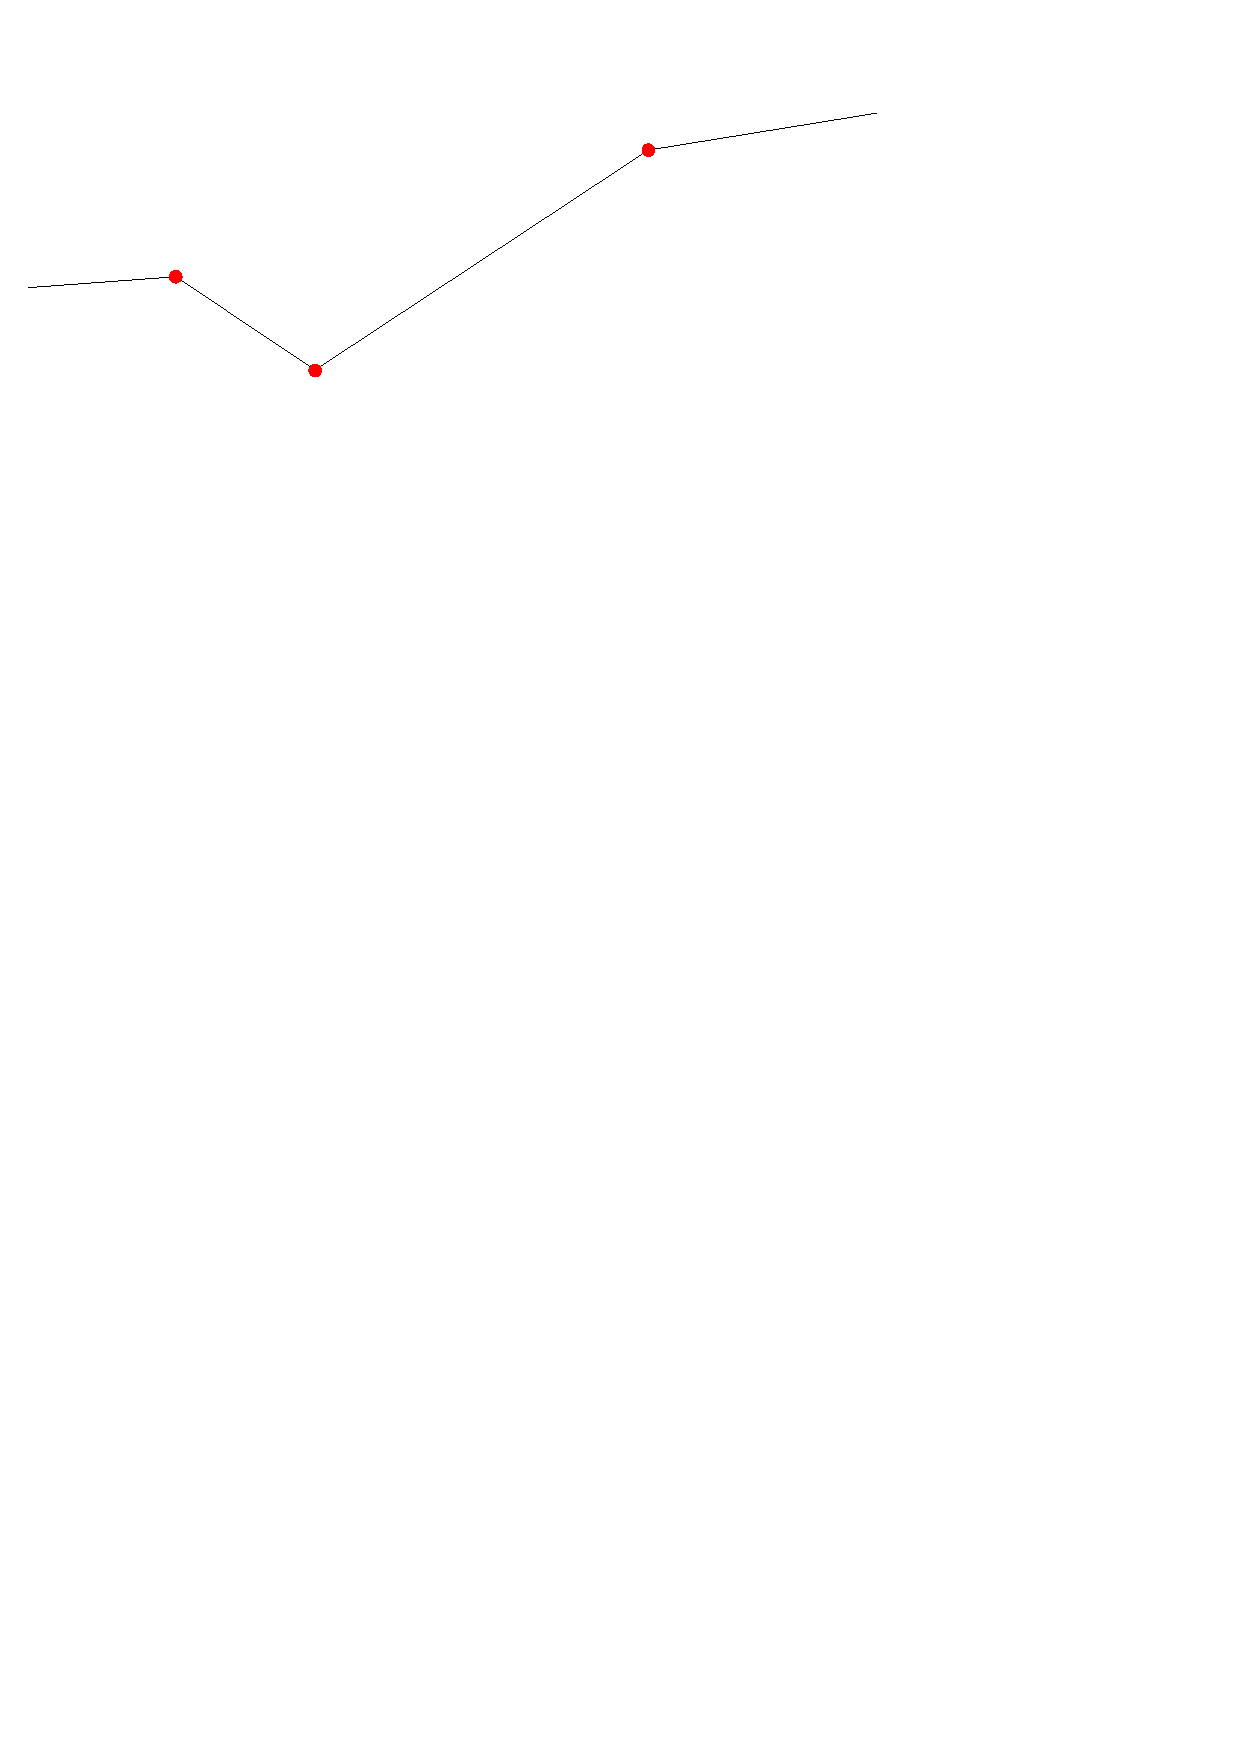
\includegraphics[width=\textwidth,page=1]{figs/1Dsmoothop.pdf}
    \caption{Initial TIN}\label{fig:1Dsmoothop:a}
  \end{subfigure}
  \quad
  \begin{subfigure}[b]{0.45\linewidth}
    \centering
    \includegraphics[width=\textwidth,page=2]{figs/1Dsmoothop.pdf}
    \caption{Estimation using only neighbours}\label{fig:1Dsmoothop:b}
  \end{subfigure}
  \quad
  \begin{subfigure}[b]{0.45\linewidth}
    \centering
    \includegraphics[width=\textwidth,page=3]{figs/1Dsmoothop.pdf}
    \caption{Comparison of depths}\label{fig:1Dsmoothop:c}
  \end{subfigure}
  \quad
  \begin{subfigure}[b]{0.45\linewidth}
    \centering
    \includegraphics[width=\textwidth,page=4]{figs/1Dsmoothop.pdf}
    \caption{Resulting TIN}\label{fig:1Dsmoothop:d}
  \end{subfigure}
  \caption{Cross-section view of the smoothing of a single vertex in a TIN.}
\label{fig:1Dsmoothop}
\end{figure}

To perform the Laplace interpolation for each vertex $v$ in the Voronoi diagram $\mathcal{D}$, it suffices to obtain the natural neighbours $p_i$ of $v$, and for each calculate the lengths of the Delaunay and the dual Voronoi edge (as explained in Section~\ref{sec:laplace}).
There is no need to insert/remove $v$ in the dataset, since we are only interested in estimating its depth (without considering the depth it is already assigned).

The primary objective of smoothing is to generalise the surface by removing high frequency detail while preserving the overall feature shape. 
Applying it reduces the angle between adjacent triangles which gives the surface a smoother look.

It performs two linear loops over the $n$ vertices of the dataset (the depths are only updated after all the depths have been estimated), and since the smoothing of one vertex is performed in expected constant time, the expected time complexity of the algorithm is $\mathcal{O}(n)$.

Observe that the operator can be performed either on a portion of a dataset, or on the whole dataset. 
Furthermore this operator can be applied any number of times, delivering more generalisation with each pass.


%%%
%
\subsubsection{The densification operator}
\label{sec:densification}

Its objective is primarily to minimise the discretisation error between the Laplace interpolated field and the contours that are extracted from the DT, this is illustrated in Figure~\ref{fig:1Ddensop}.
\begin{figure}
  \centering
  \begin{subfigure}[b]{0.35\linewidth}
    \centering
    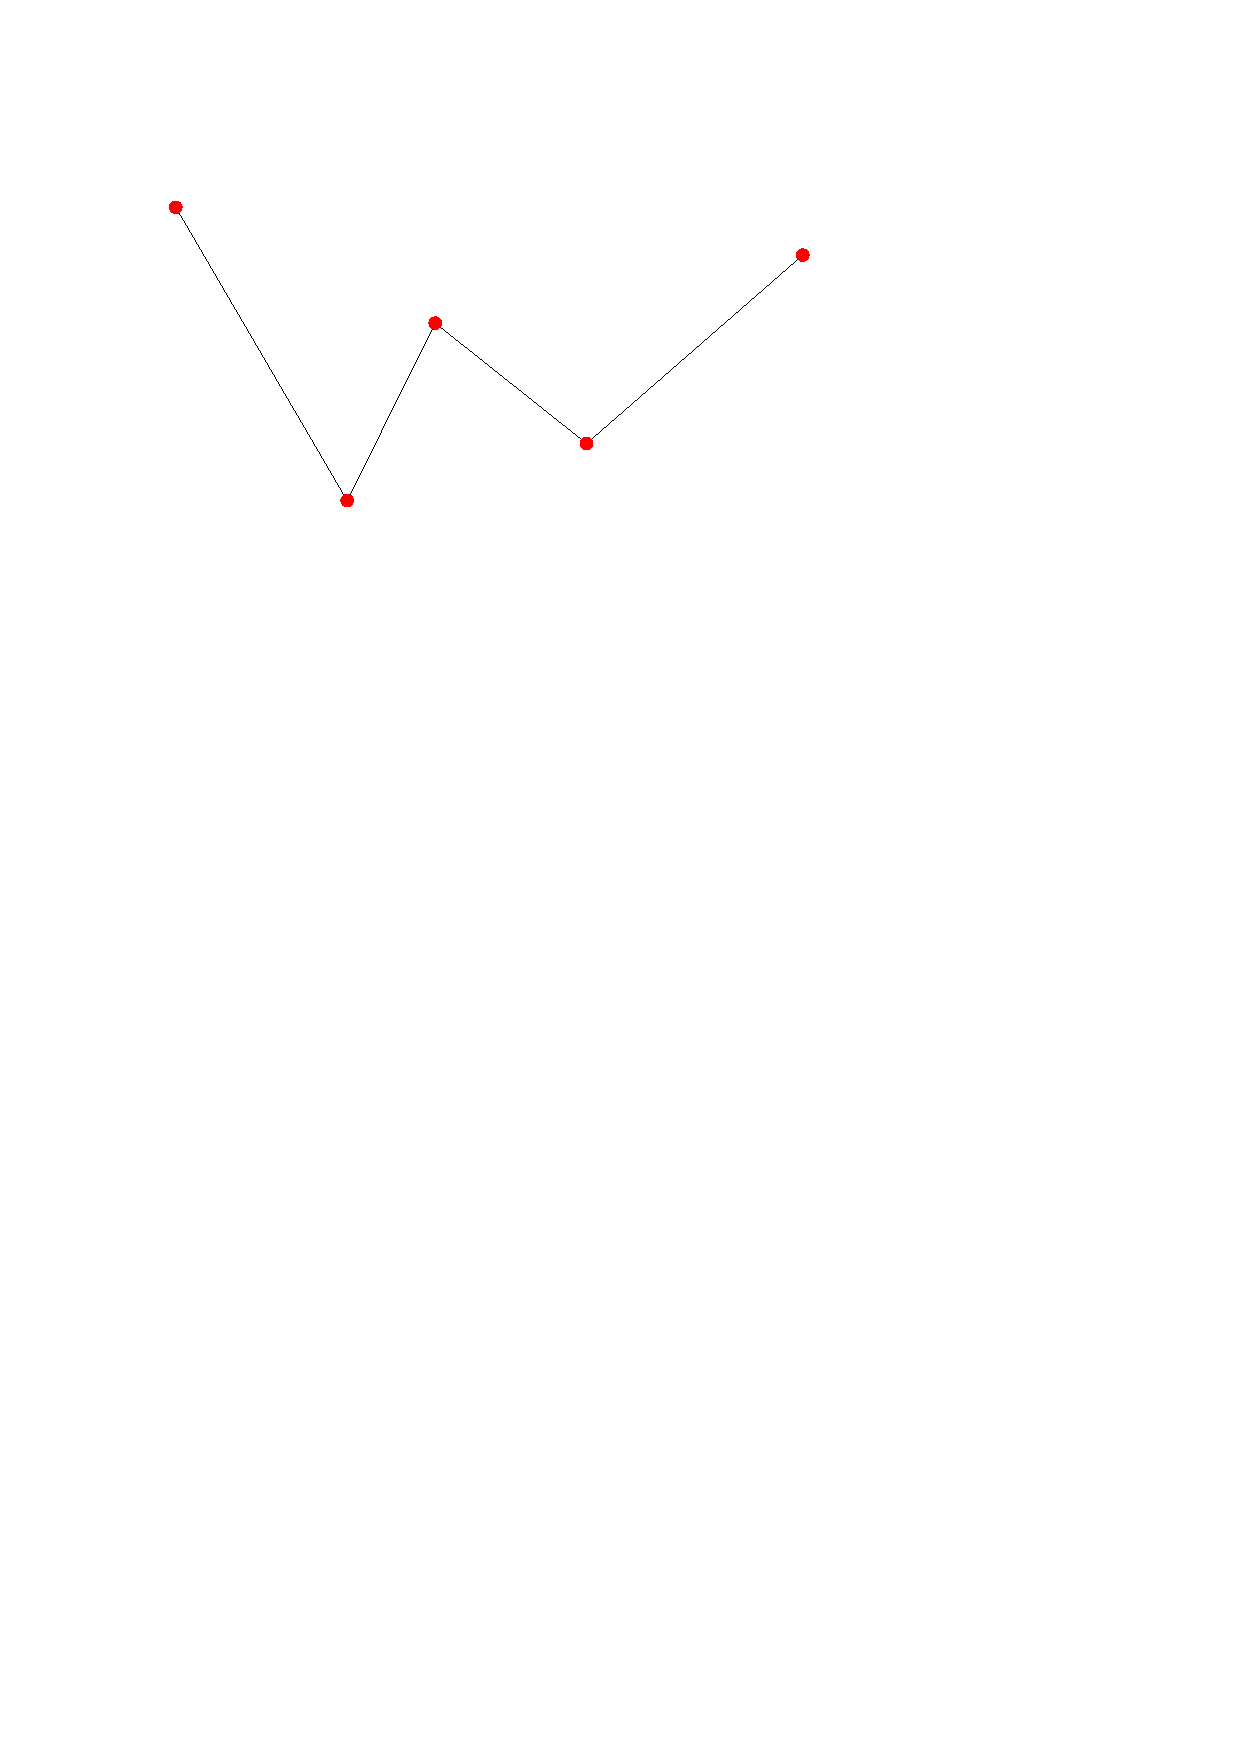
\includegraphics[width=\textwidth,page=1]{figs/1Ddensop.pdf}
    \caption{Initial TIN}\label{fig:1Ddensop:a}
  \end{subfigure}
  \quad
  \begin{subfigure}[b]{0.35\linewidth}
    \centering
    \includegraphics[width=\textwidth,page=2]{figs/1Ddensop.pdf}
    \caption{Interpolated field (dashed)}\label{fig:1Ddensop:b}
  \end{subfigure}
  \quad
  \begin{subfigure}[b]{0.35\linewidth}
    \centering
    \includegraphics[width=\textwidth,page=3]{figs/1Ddensop.pdf}
    \caption{Addition of intermediate points (orange)}\label{fig:1Ddensop:c}
  \end{subfigure}
  \quad
  \begin{subfigure}[b]{0.35\linewidth}
    \centering
    \includegraphics[width=\textwidth,page=4]{figs/1Ddensop.pdf}
    \caption{Resulting TIN}\label{fig:1Ddensop:d}
  \end{subfigure}
  \caption{Cross-section view of the densification operator in a TIN.}
\label{fig:1Ddensop}
\end{figure}

By inserting extra vertices in large triangles (to break them into three triangles), the resolution of the DT is improved.
As a result also the extracted contour lines have a smoother appearance because they now have shorter line-segments; see Section~\ref{sec:smoothness-contours} for an explanation.
We insert a new vertex at the centre of the circumscribed circle of any triangle that has an area greater than a preset threshold; its depth is assigned with the Laplace interpolant.
The circumcentre is chosen here because that location is equidistant to its three closest points, and subsequently results in a very natural point distribution.

%

Figure~\ref{fig:interpol_smooth}
\begin{figure}
  \centering
  \begin{subfigure}[b]{0.3\linewidth}
    \centering
    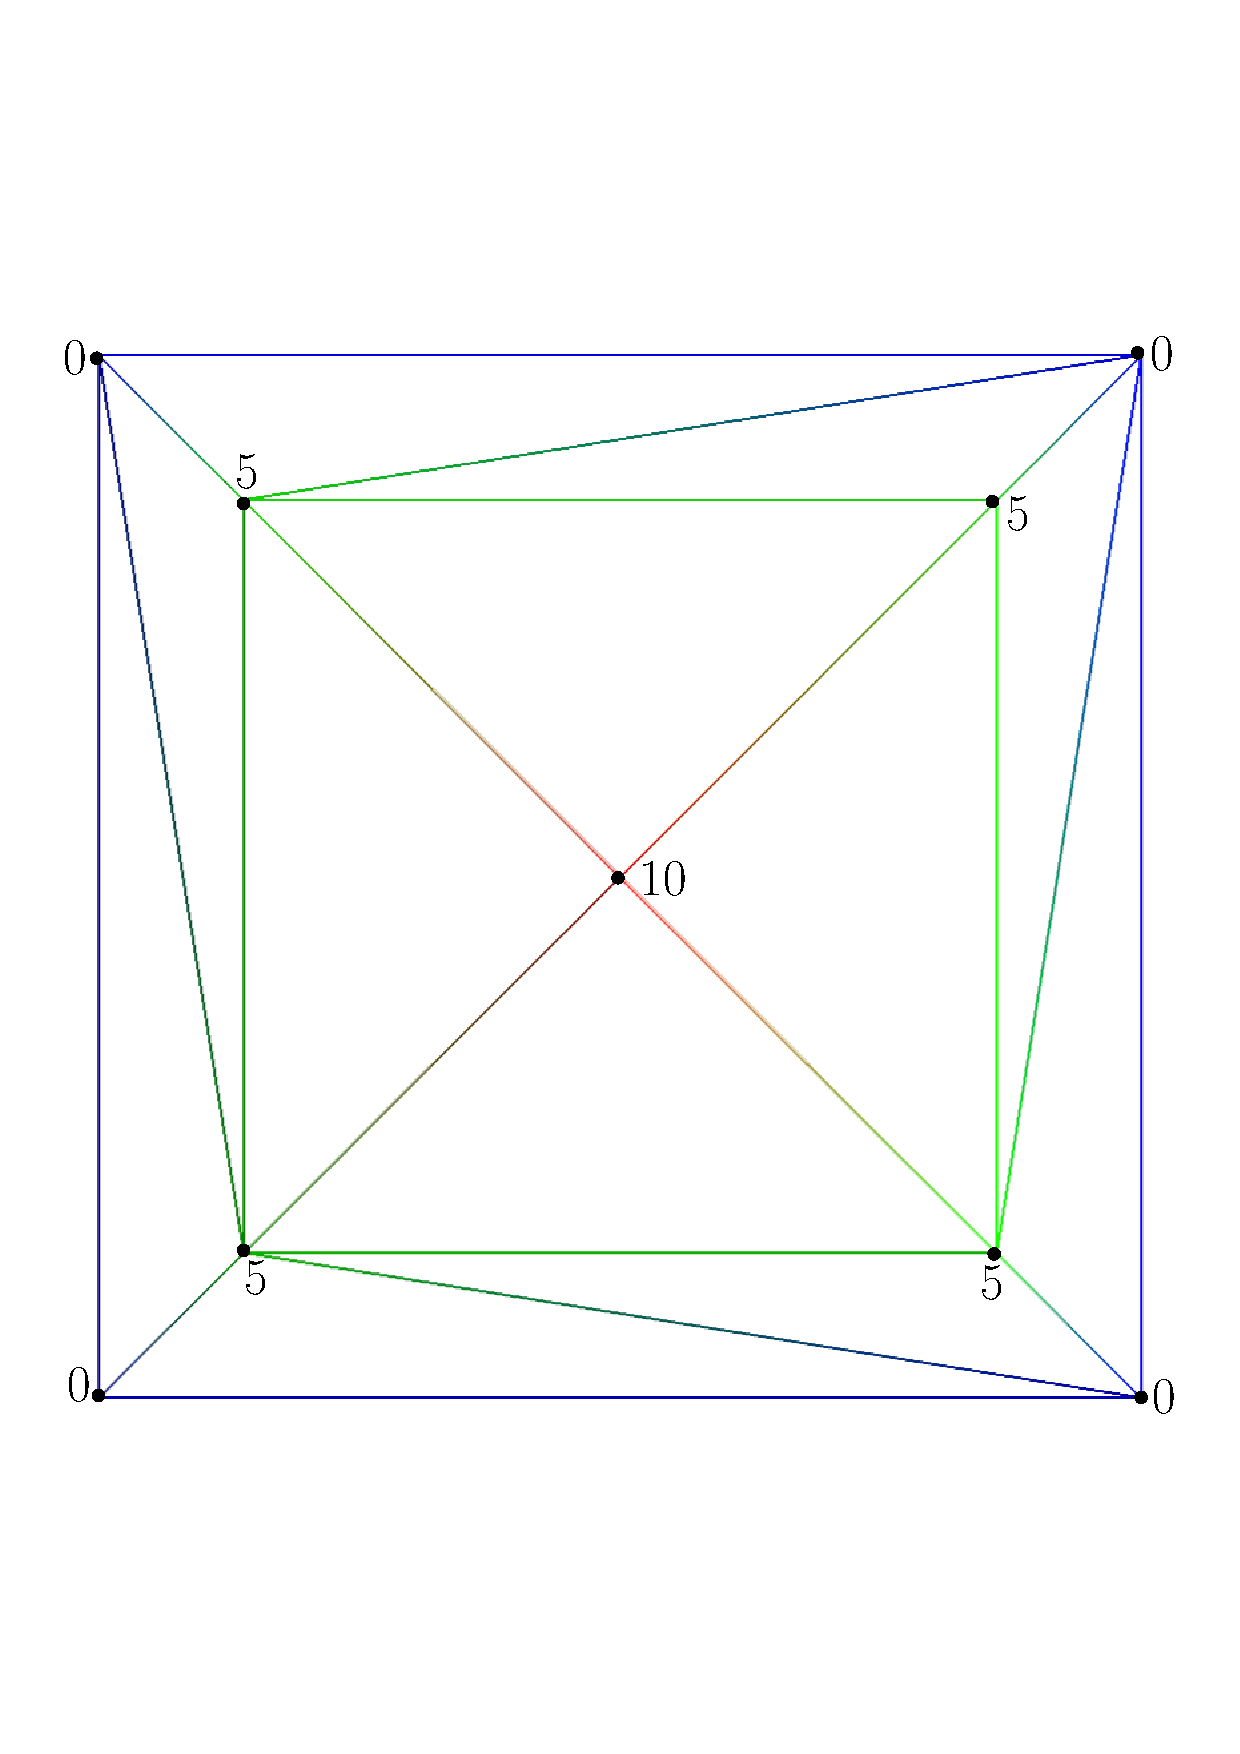
\includegraphics[width=\textwidth]{figs/pyramid_o_tr}
    \caption{Original data}
  \end{subfigure}  
  \quad
  \begin{subfigure}[b]{0.3\linewidth}
    \centering
    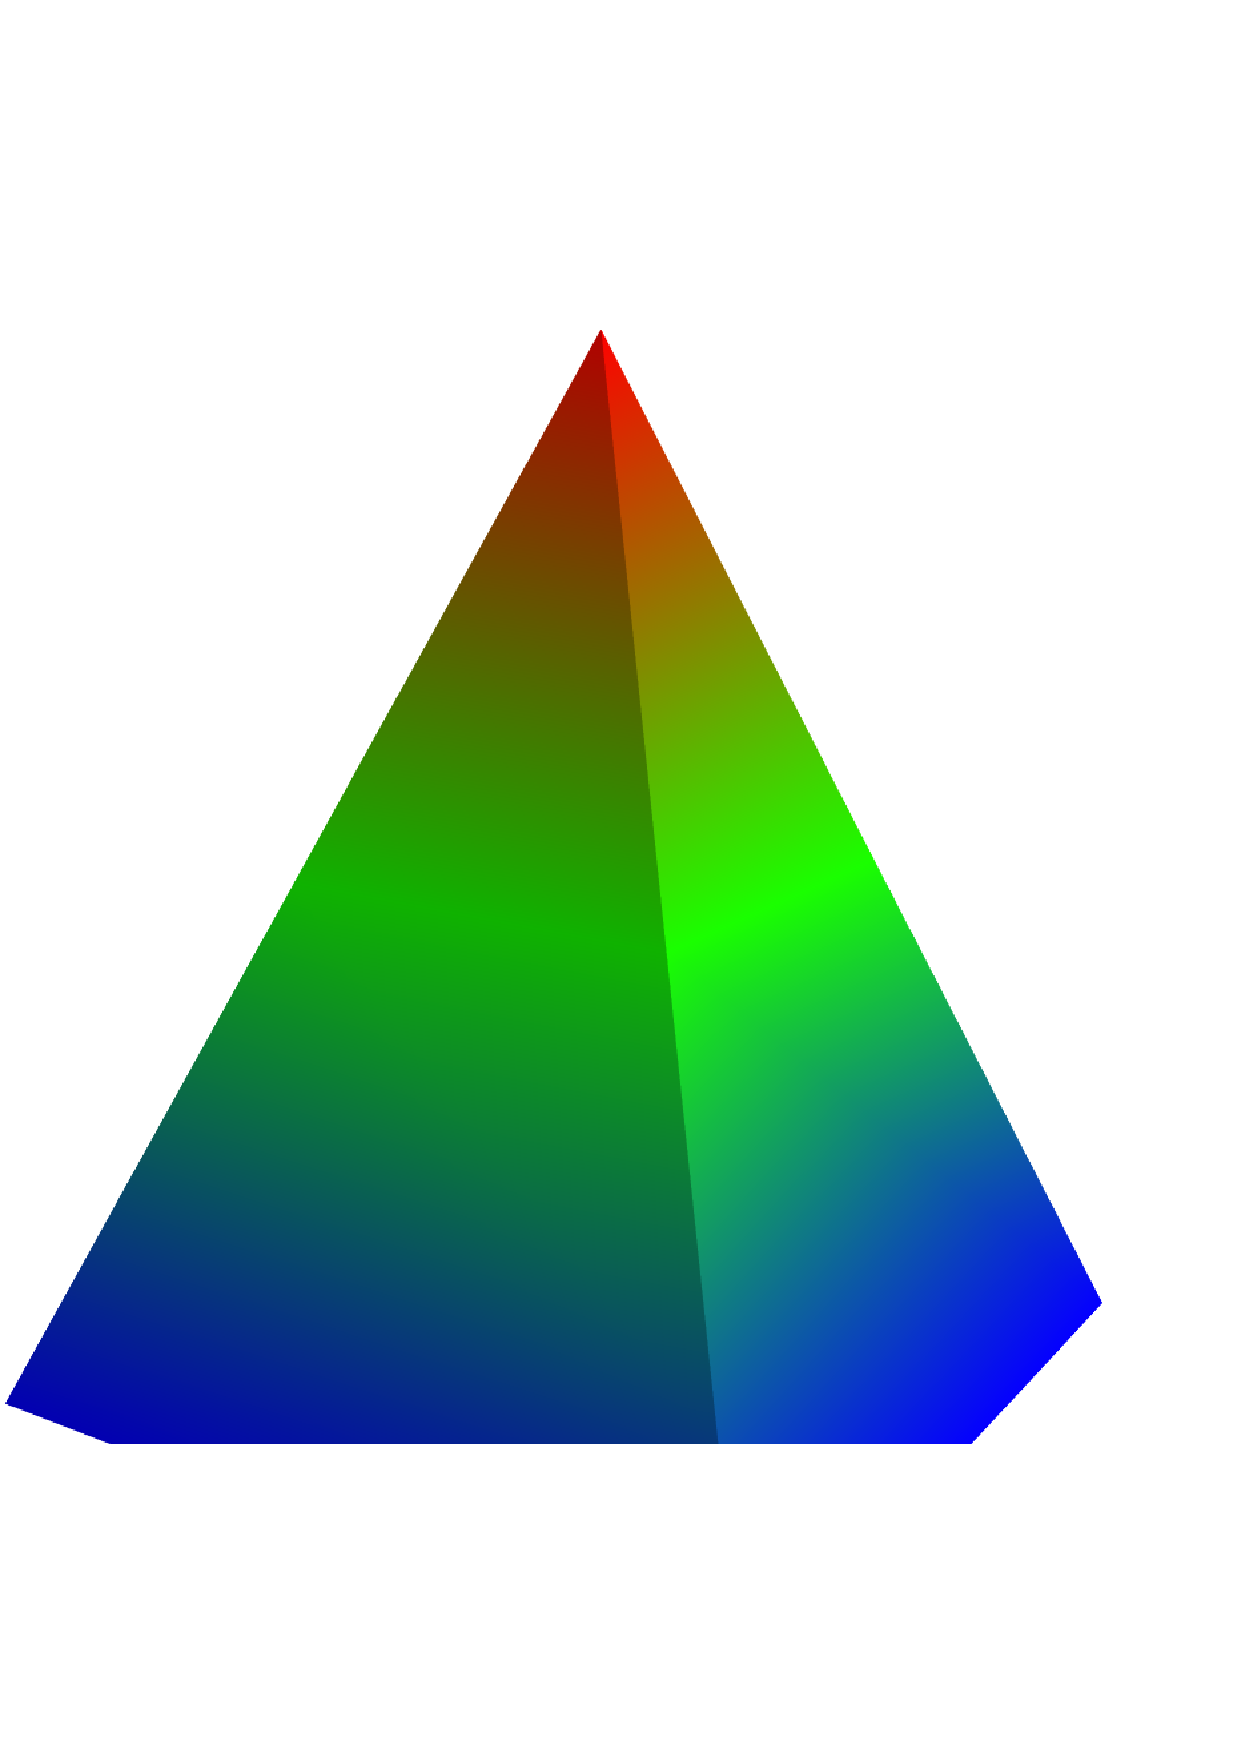
\includegraphics[width=\textwidth]{figs/pyramid_o_pers}
    \caption{Perspective view of original data}
  \end{subfigure}  
  \quad
  \begin{subfigure}[b]{0.3\linewidth}
    \centering
    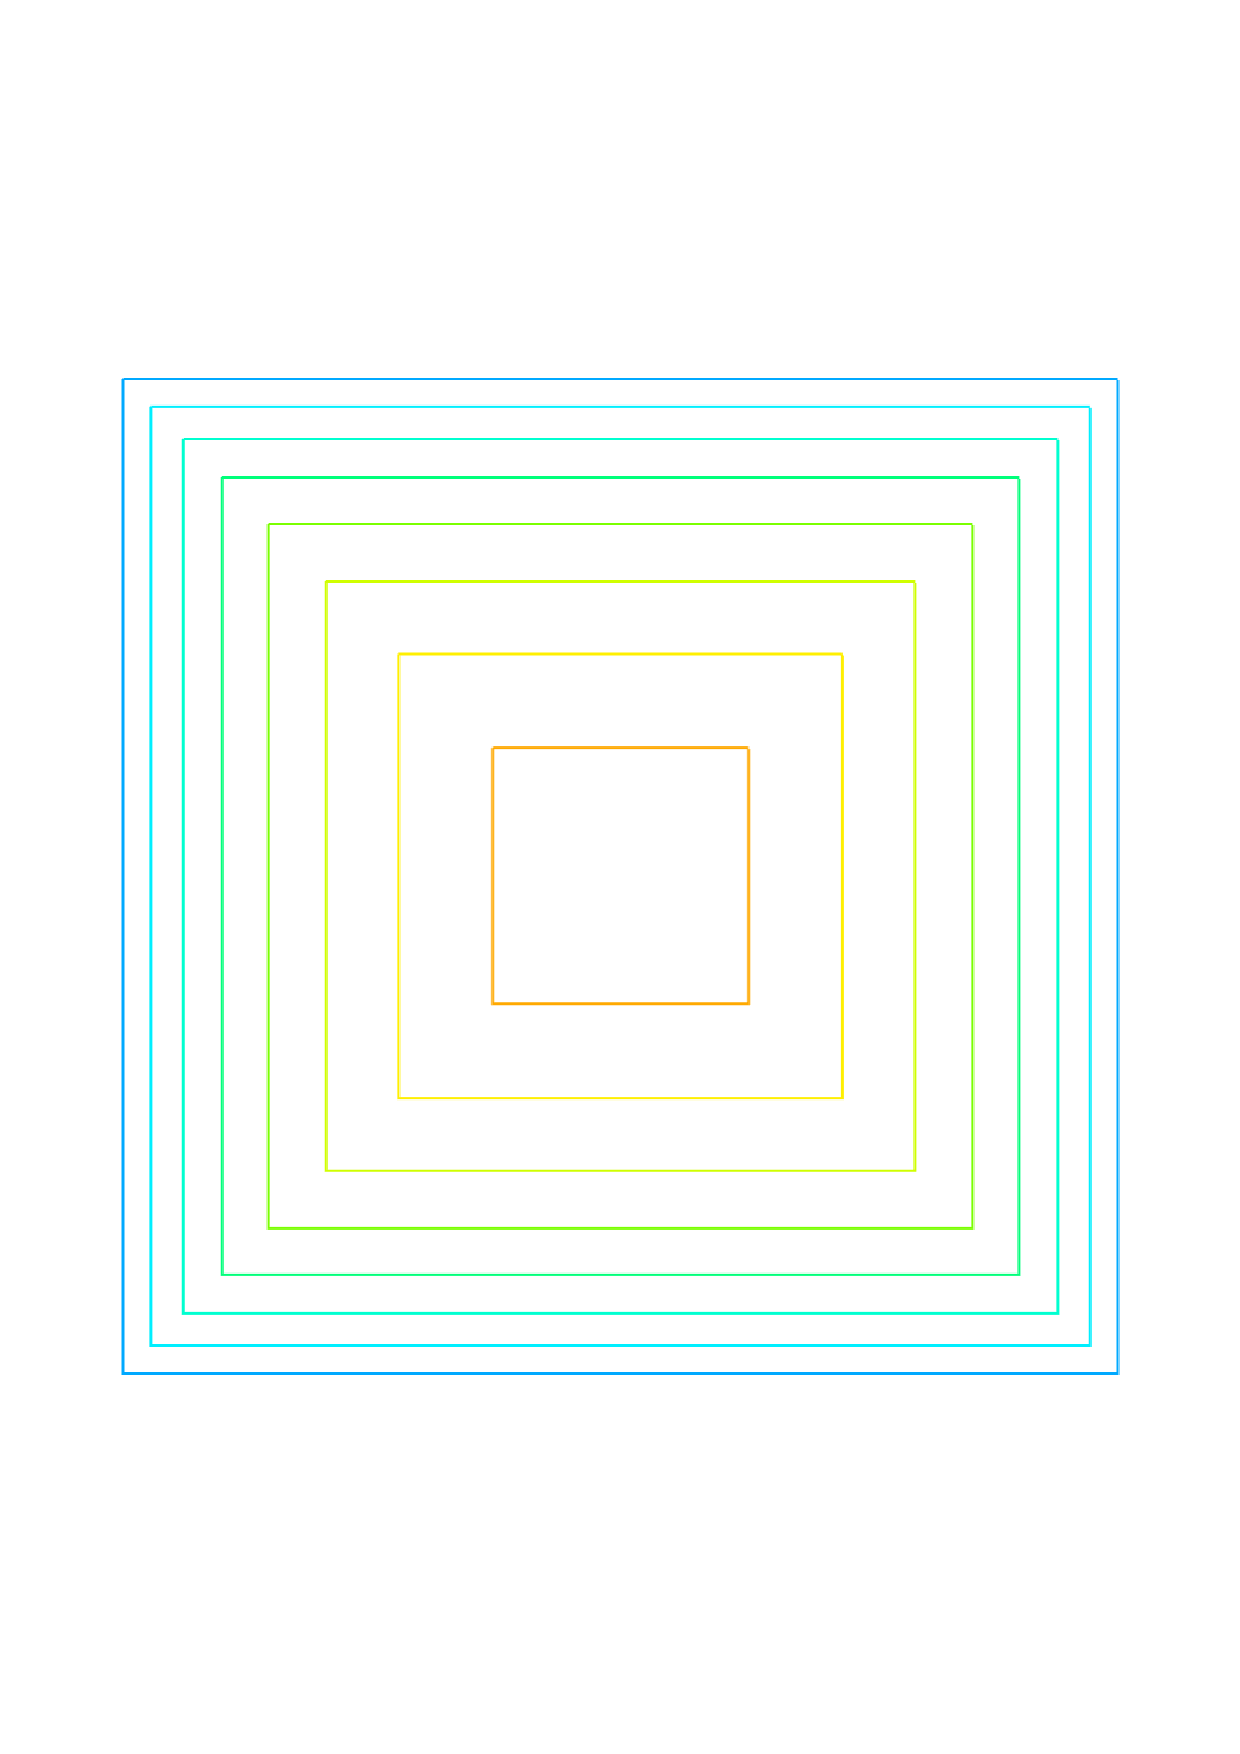
\includegraphics[width=\textwidth]{figs/pyramid_o_cl}
    \caption{Contour lines from original data}
  \end{subfigure}  
  \quad
  \begin{subfigure}[b]{0.3\linewidth}
    \centering
    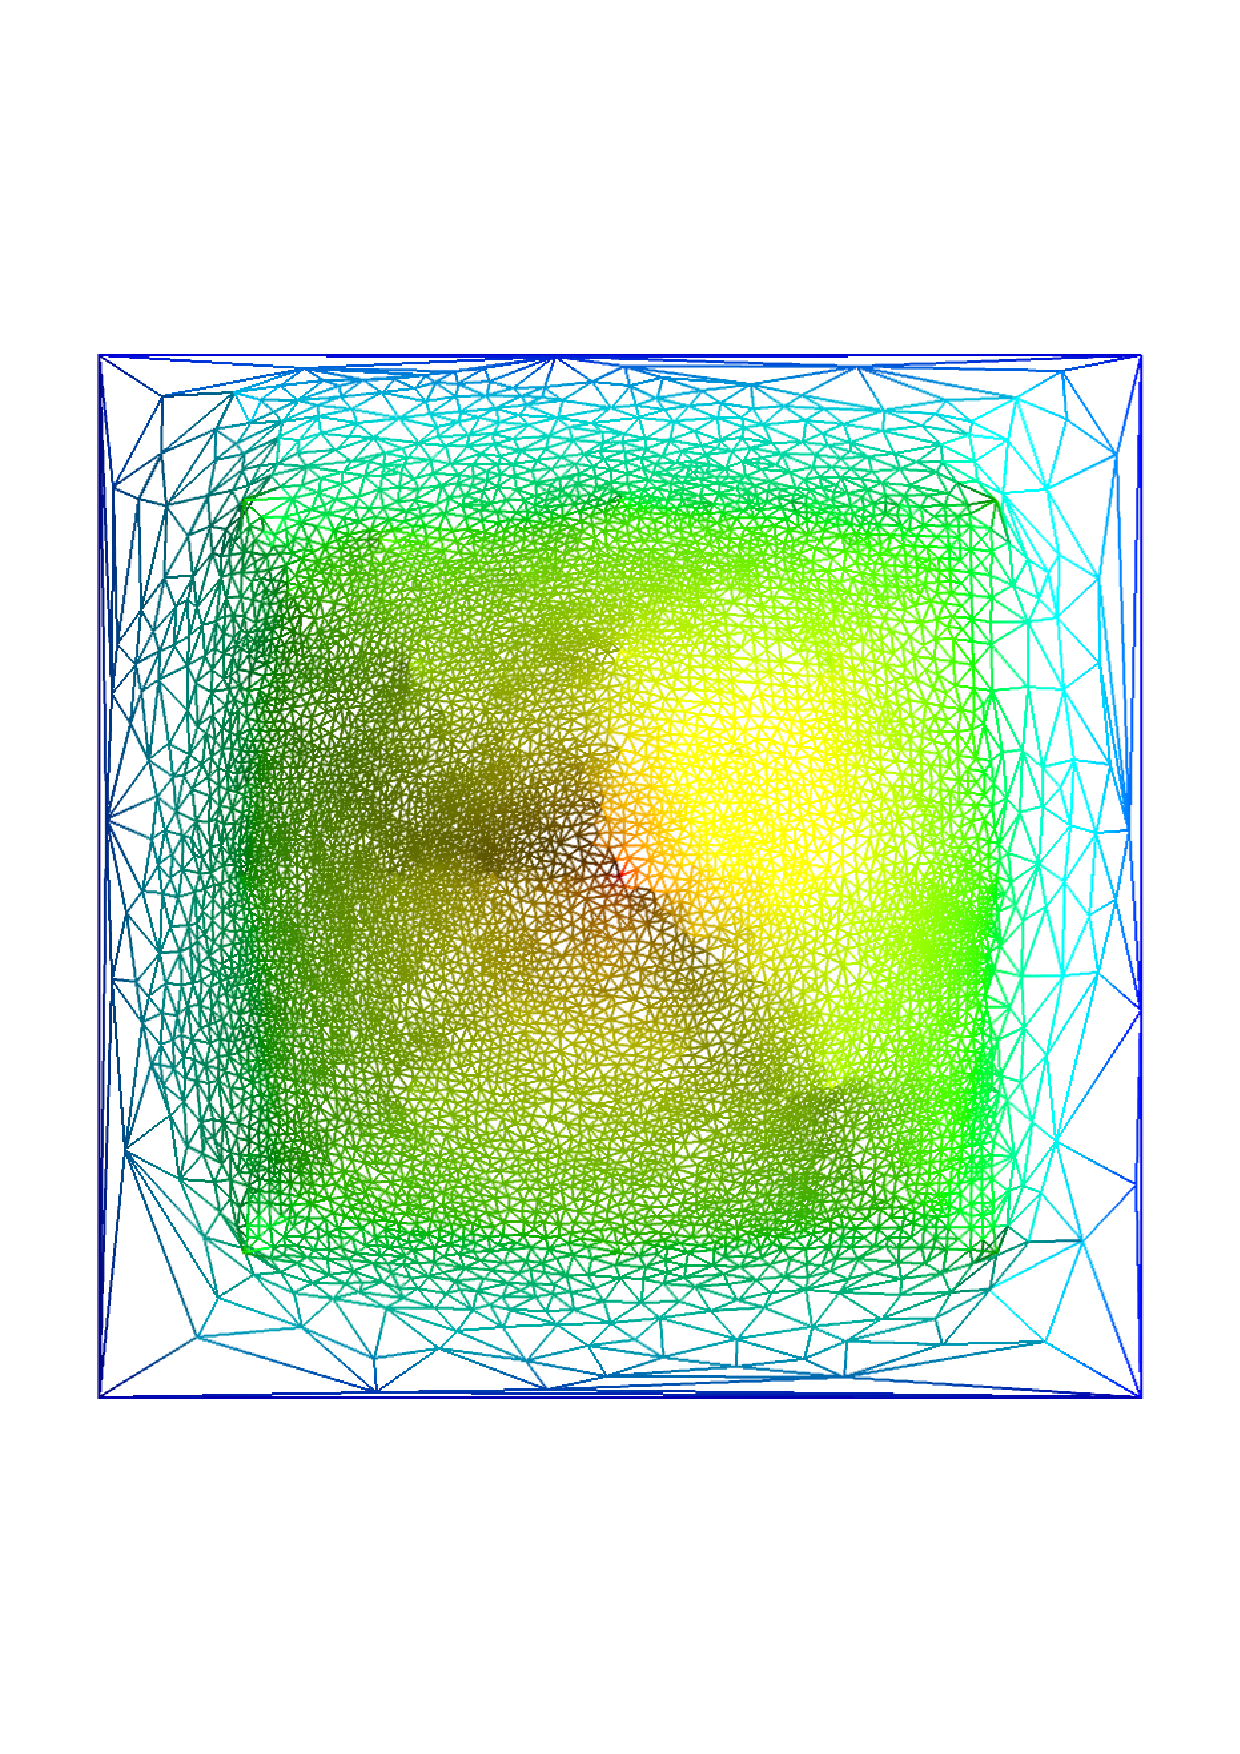
\includegraphics[width=\textwidth]{figs/pyramid_v_tr}
    \caption{Densified with Laplace interpolant}
  \end{subfigure}  
  \quad
  \begin{subfigure}[b]{0.3\linewidth}
    \centering
    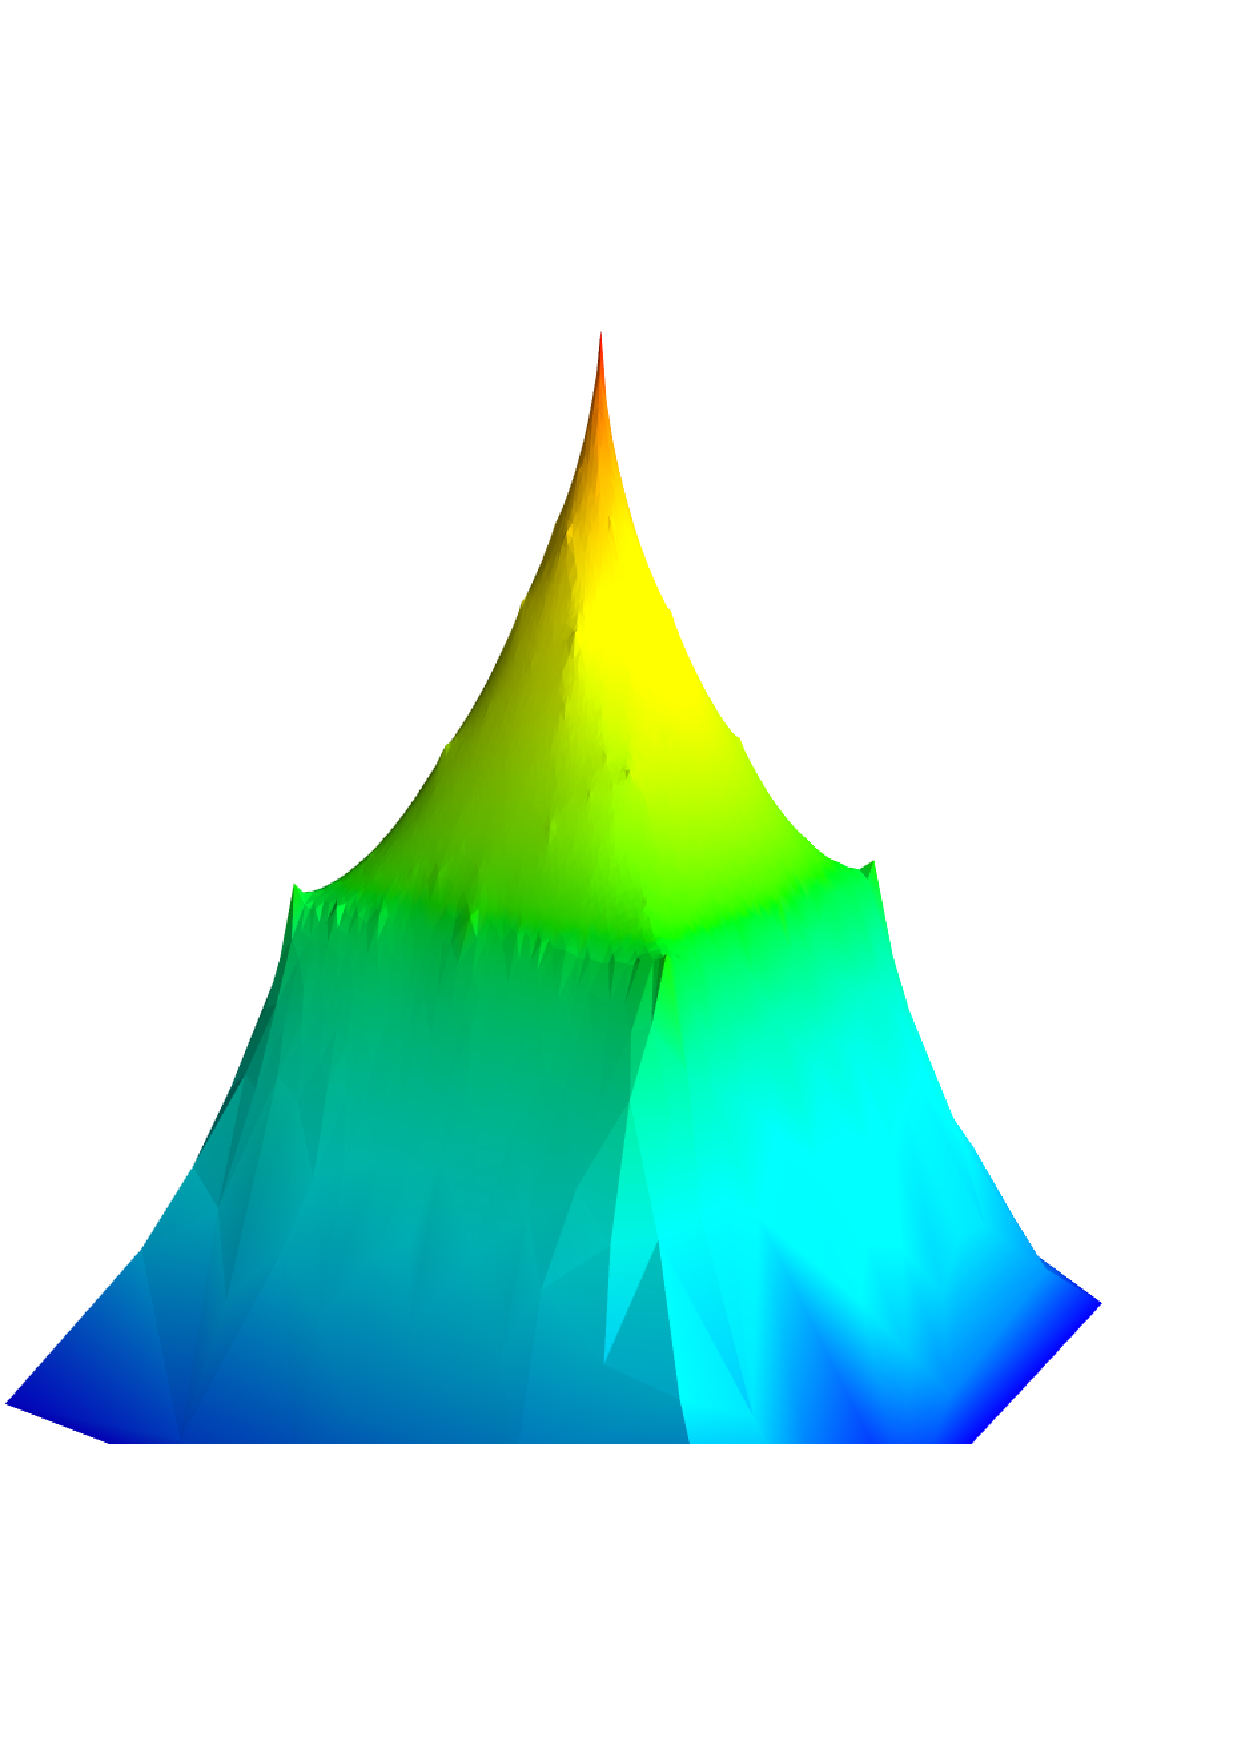
\includegraphics[width=\textwidth]{figs/pyramid_v_pers}
    \caption{Perspective view after densification}
  \end{subfigure}  
  \quad
  \begin{subfigure}[b]{0.3\linewidth}
    \centering
    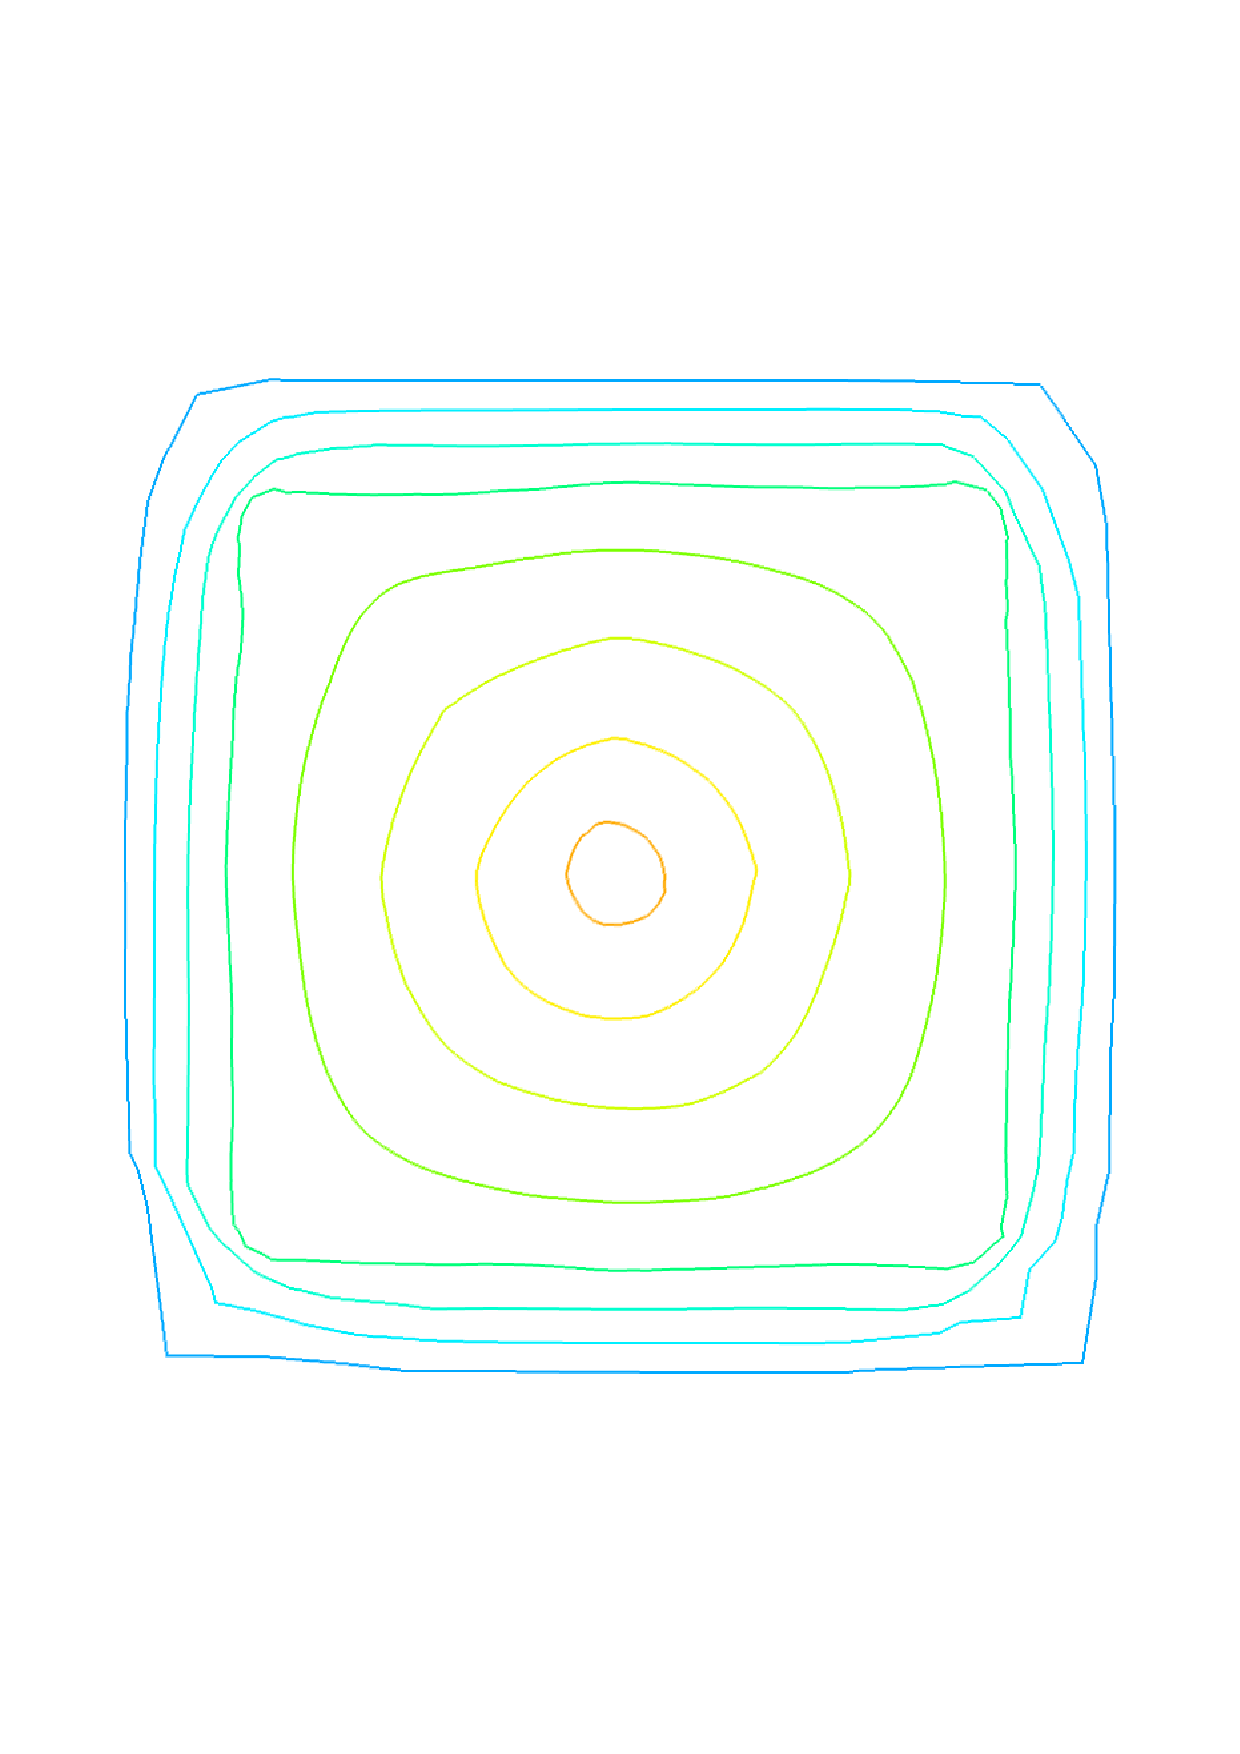
\includegraphics[width=\textwidth]{figs/pyramid_v_cl}
    \caption{Contour lines from densified surface}
  \end{subfigure}  
  \caption{Original data are shown in \textbf{(a)} and \textbf{(b)}, and the resulting contour lines in \textbf{(c)}. The three figures below represent the same area densified with the Laplace interpolant.}
\label{fig:interpol_smooth}
\end{figure}
shows an example of these ideas. 
Figure~\ref{fig:interpol_smooth}a and Figure~\ref{fig:interpol_smooth}b show the original dataset, which is a very simple pyramid having its base at elevation 0, and its summit at 10. 
Figure~\ref{fig:interpol_smooth}d--f shows the results when a densification operator based on the Laplace interpolant is used. 
It should be noticed that the ``top'' of the pyramid was densified, and not so much the bottom, therefore the contour lines near the bottom should be ignored (the fact that they are close to the border of the dataset also creates artefacts).


%

Densification aims to improve the reduce the difference between the linear TIN and the Laplace interpolated field of its vertices---effectively improving the resolution of the extracted contours.
Therefore, densification is to be applied just before the extraction of the depth-contours.
If applied \emph{before} the smoothing operator, it would limit the effectiveness of that operator, since a denser triangulation smoothes more slowly.

The densification operator uses an area-threshold that determines which triangles should be densified. 
This way triangles that are already sufficiently small are not densified. 
It performs a single pass on the input triangles, thus with every call the resolution of the DT is increased, until all triangles have reached a certain area.

If the maximum area threshold is ignored, a single call to costs $\mathcal{O}(n)$ time, as it only requires a single pass over the $n$ triangles of the TIN\@. 
However, when a number of $t$ densification passes is sequentially performed, it only scales to $\mathcal{O}(3^t \, n)$ time, since every point insertion creates two new triangles. 
However, because of the maximum area threshold, that worst case scenario will never be reached in practice with large $t$.


%%%
%
\section{Some examples of results with real-world datasets}


Figure~\ref{fig:zl1845fieldview} shows the results obtained with the implementation of the method described in this chapter.
This was tested with an MBES dataset from Zeeland, in the Netherlands.
\begin{figure}
\centering
  \begin{subfigure}[b]{0.55\linewidth}
    \centering
    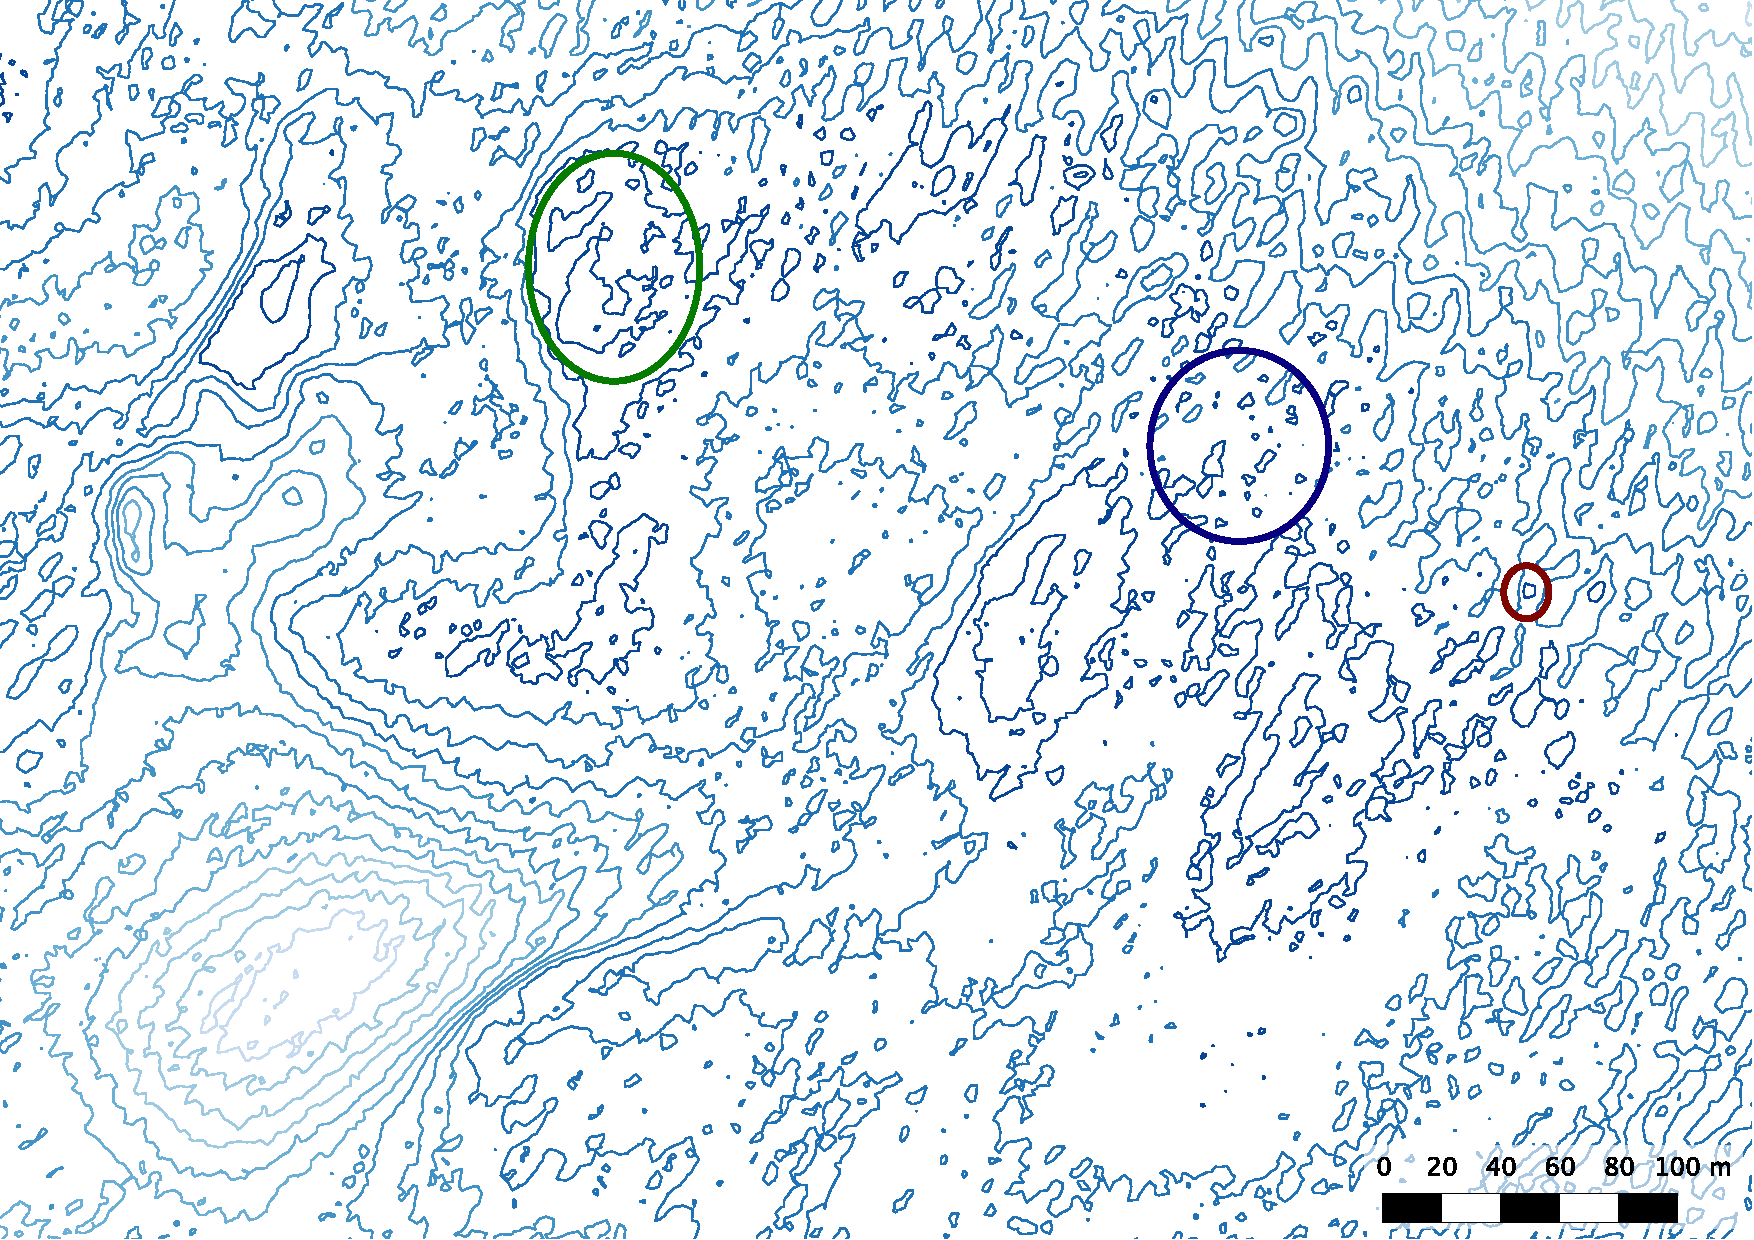
\includegraphics[width=\textwidth]{figs/zl1845fieldview_o.pdf}
    \caption{}\label{fig:zl1845fieldview_o}
  \end{subfigure}
  \quad
  \begin{subfigure}[b]{0.55\linewidth}
    \centering
    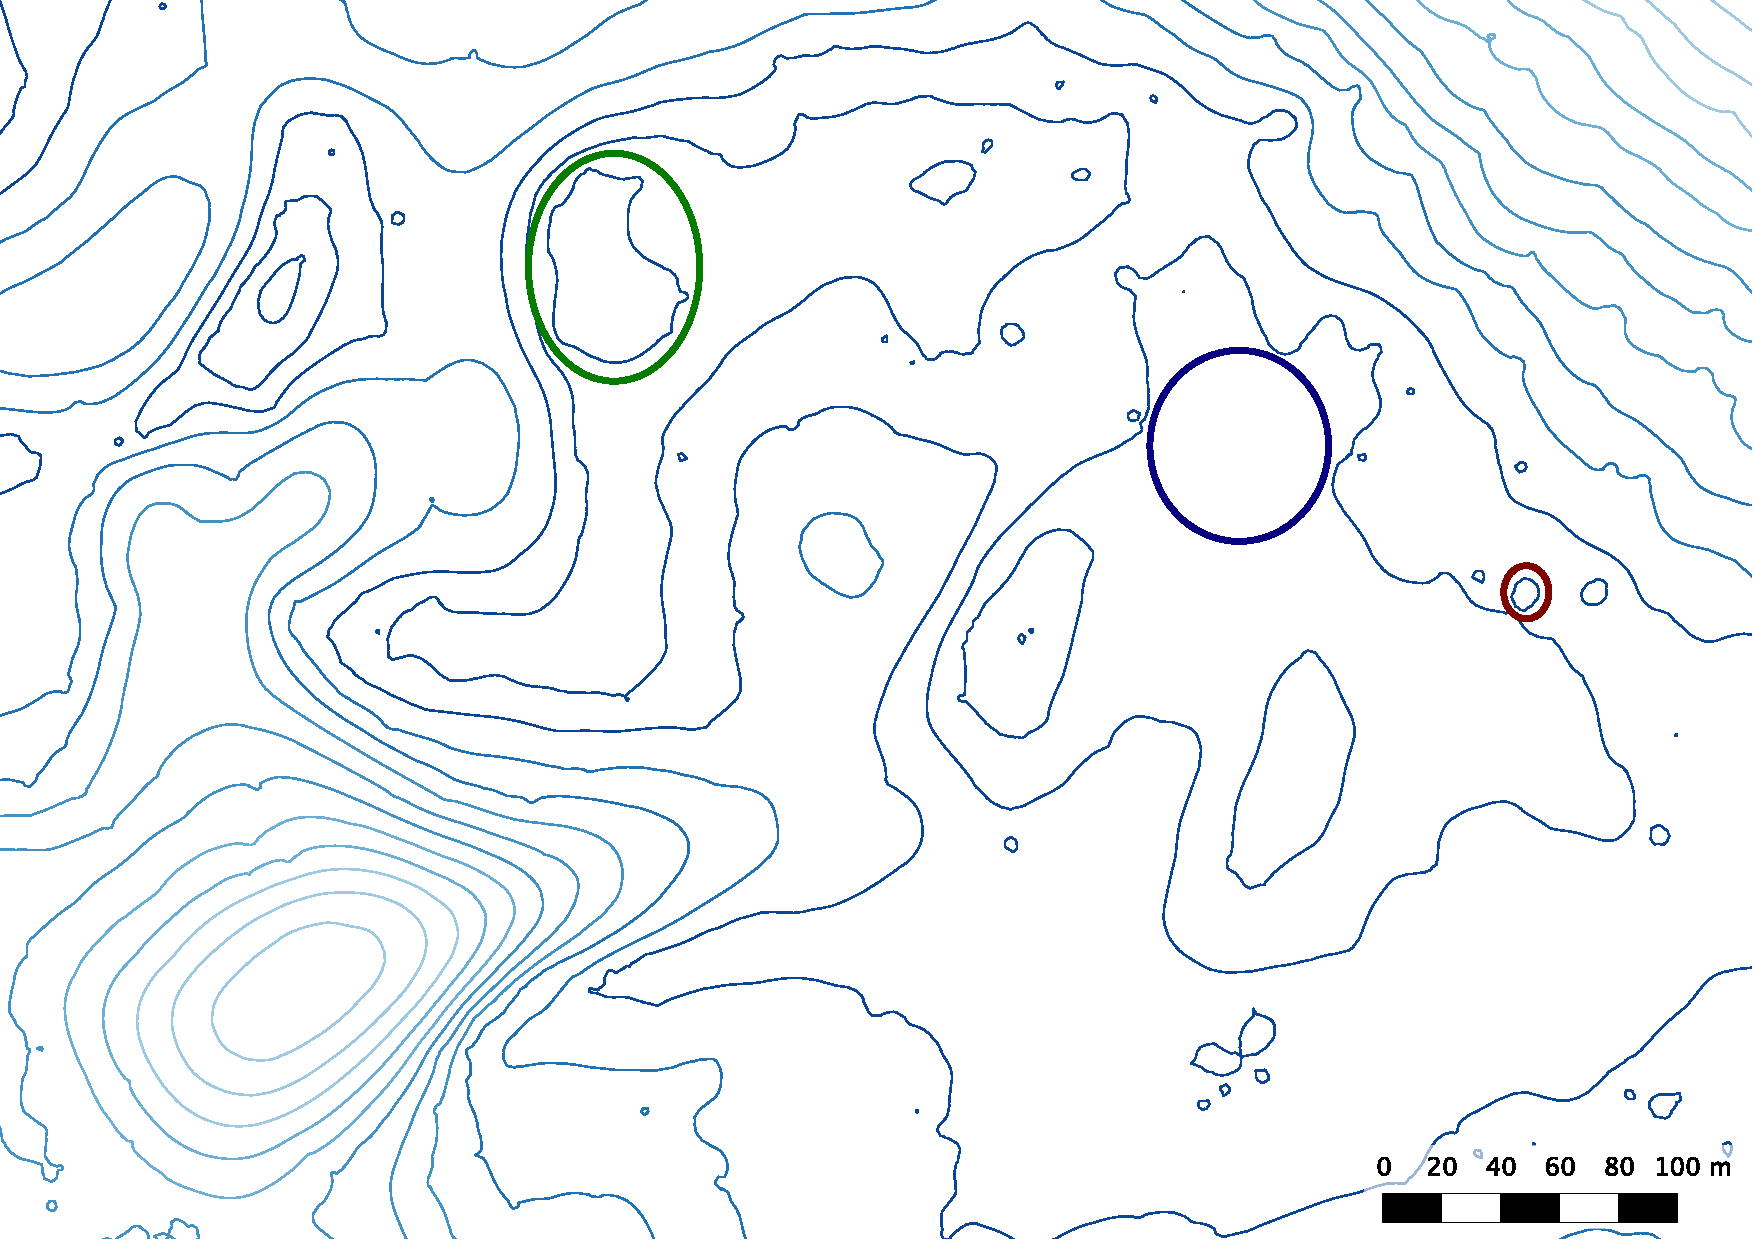
\includegraphics[width=\textwidth]{figs/zl1845fieldview_s.pdf}
    \caption{}\label{fig:zl1845fieldview_s}
  \end{subfigure}
  \quad
  \begin{subfigure}[b]{0.55\linewidth}
    \centering
    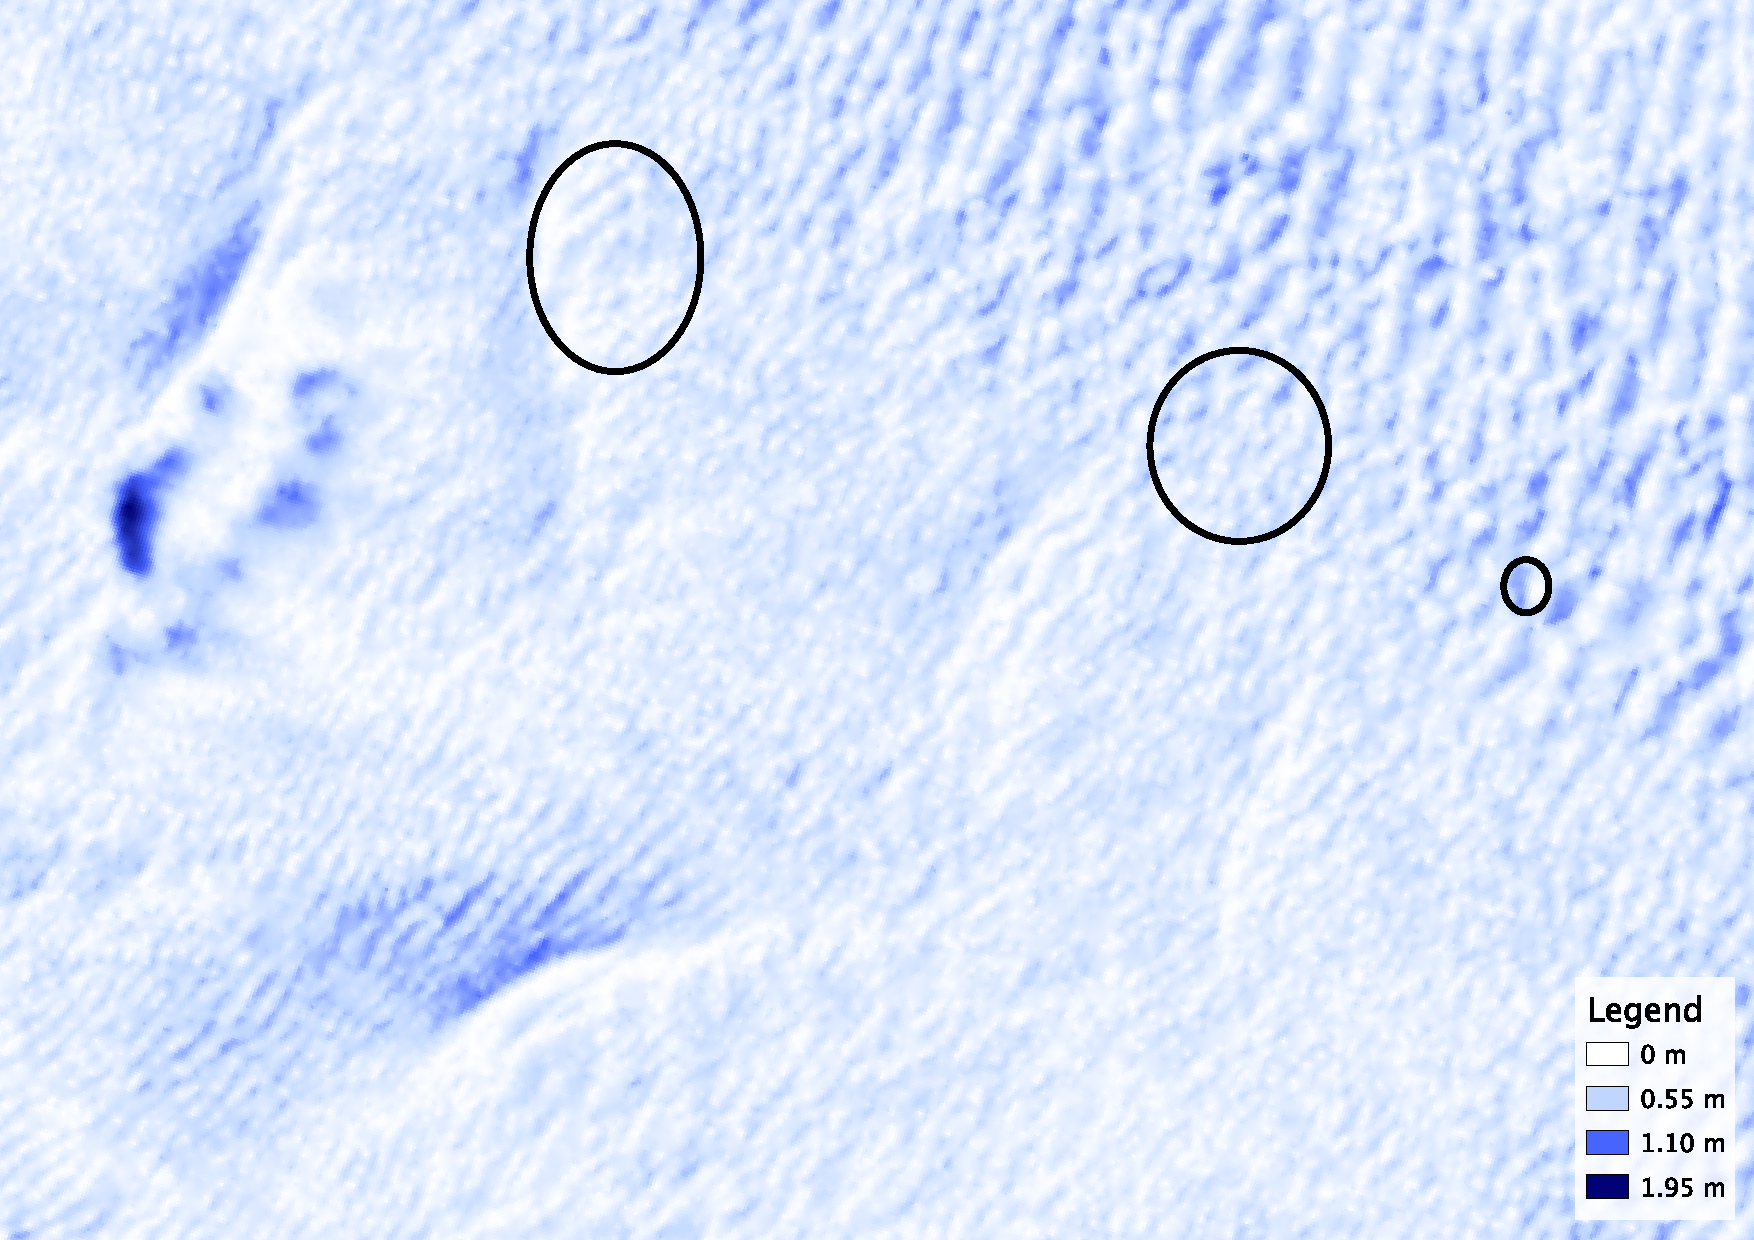
\includegraphics[width=\textwidth]{figs/zl1845fieldview_raster_d.pdf}
    \caption{}\label{fig:zl1845fieldview_raster_d}
  \end{subfigure}
  \quad
  % \begin{subfigure}[b]{0.45\linewidth}
    % \centering
    % 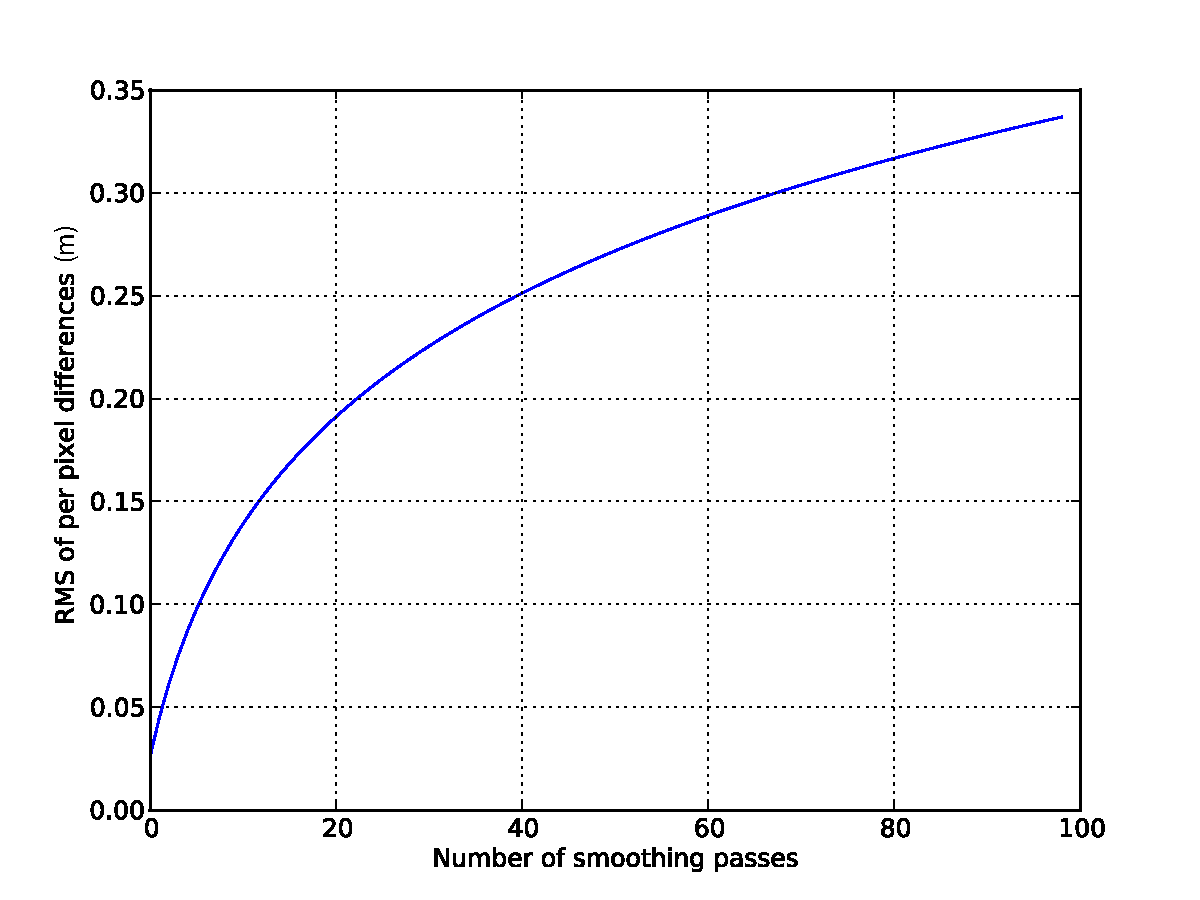
\includegraphics[width=\textwidth]{figs/zl1845rmsdiffplot.pdf}
    % \caption{}\label{fig:zl1845rmsdiffplot}
  % \end{subfigure}
  \caption{The effect of the smoothing operator in the Zeeland dataset. \textbf{(a)} Raw contours extracted at a 50cm depth interval. \textbf{(b)} Smoothed contours (100 smoothing passes). The ellipses mark areas where aggregation (left), omission (middle) and enlargement (right) take place. \textbf{(c)} Difference map between the initial and 100X smoothed interpolated and rasterised fields (pixelsize 50 cm).}
\label{fig:zl1845fieldview}
\end{figure}
As can be observed from Figure~\ref{fig:zl1845fieldview_o}, the raw and ungeneralised contours in the dataset have a very irregular and cluttered appearance. 
However, the smoothed contours (100 smoothing passes) from Figure~\ref{fig:zl1845fieldview_s} have a much cleaner and less cluttered appearance. 
Clearly, the number of contour lines has diminished. 
This is both because pits (local minima) have been lifted upwards by the smoothing operator, and nearby peaks (local maxima) have been aggregated (because the region in-between has been lifted upwards). 
Notice also that a third effect of the smoothing operator is the enlargement of certain features as a result of the uplifting of the points surrounding a local maximum. 

%

% As to be expected, the overall effect of the smoothing operator on the morphology of the surface is significant.
% As shown by the plot of the root mean square (RMS) error between the initial and the generalised field in Figure~\ref{fig:zl1845rmsdiffplot}, the smoothing of the surface is most significant in the earlier smoothing passes and results in a per pixel difference of tens of centimetres.
% That supports the idea that the smoothing of the surface works against the preservation of \emph{all} morphological features. 
% However, from the difference map in Figure~\ref{fig:zl1845fieldview_raster_d}, it can be seen that the high frequency features are especially altered, thus preserving the general surface shape (low frequency pattern). 

%

The effects of the densification operator are also visible. 
The sharp edges of the undensified lines are caused by the large triangles in the initial TIN, however after densification these large triangles are subdivided into much smaller ones. 
The result is a much smoother contour line that still respects the sample points. 


%


Naturally, the smoothing operator also smoothes and simplifies the resulting contour lines. 
This is demonstrated in Figure~\ref{fig:zl1845lineview} illustrates the effect of the smoothing operator on a single contour over 30 smoothing passes. 
\begin{figure}
  \centering
  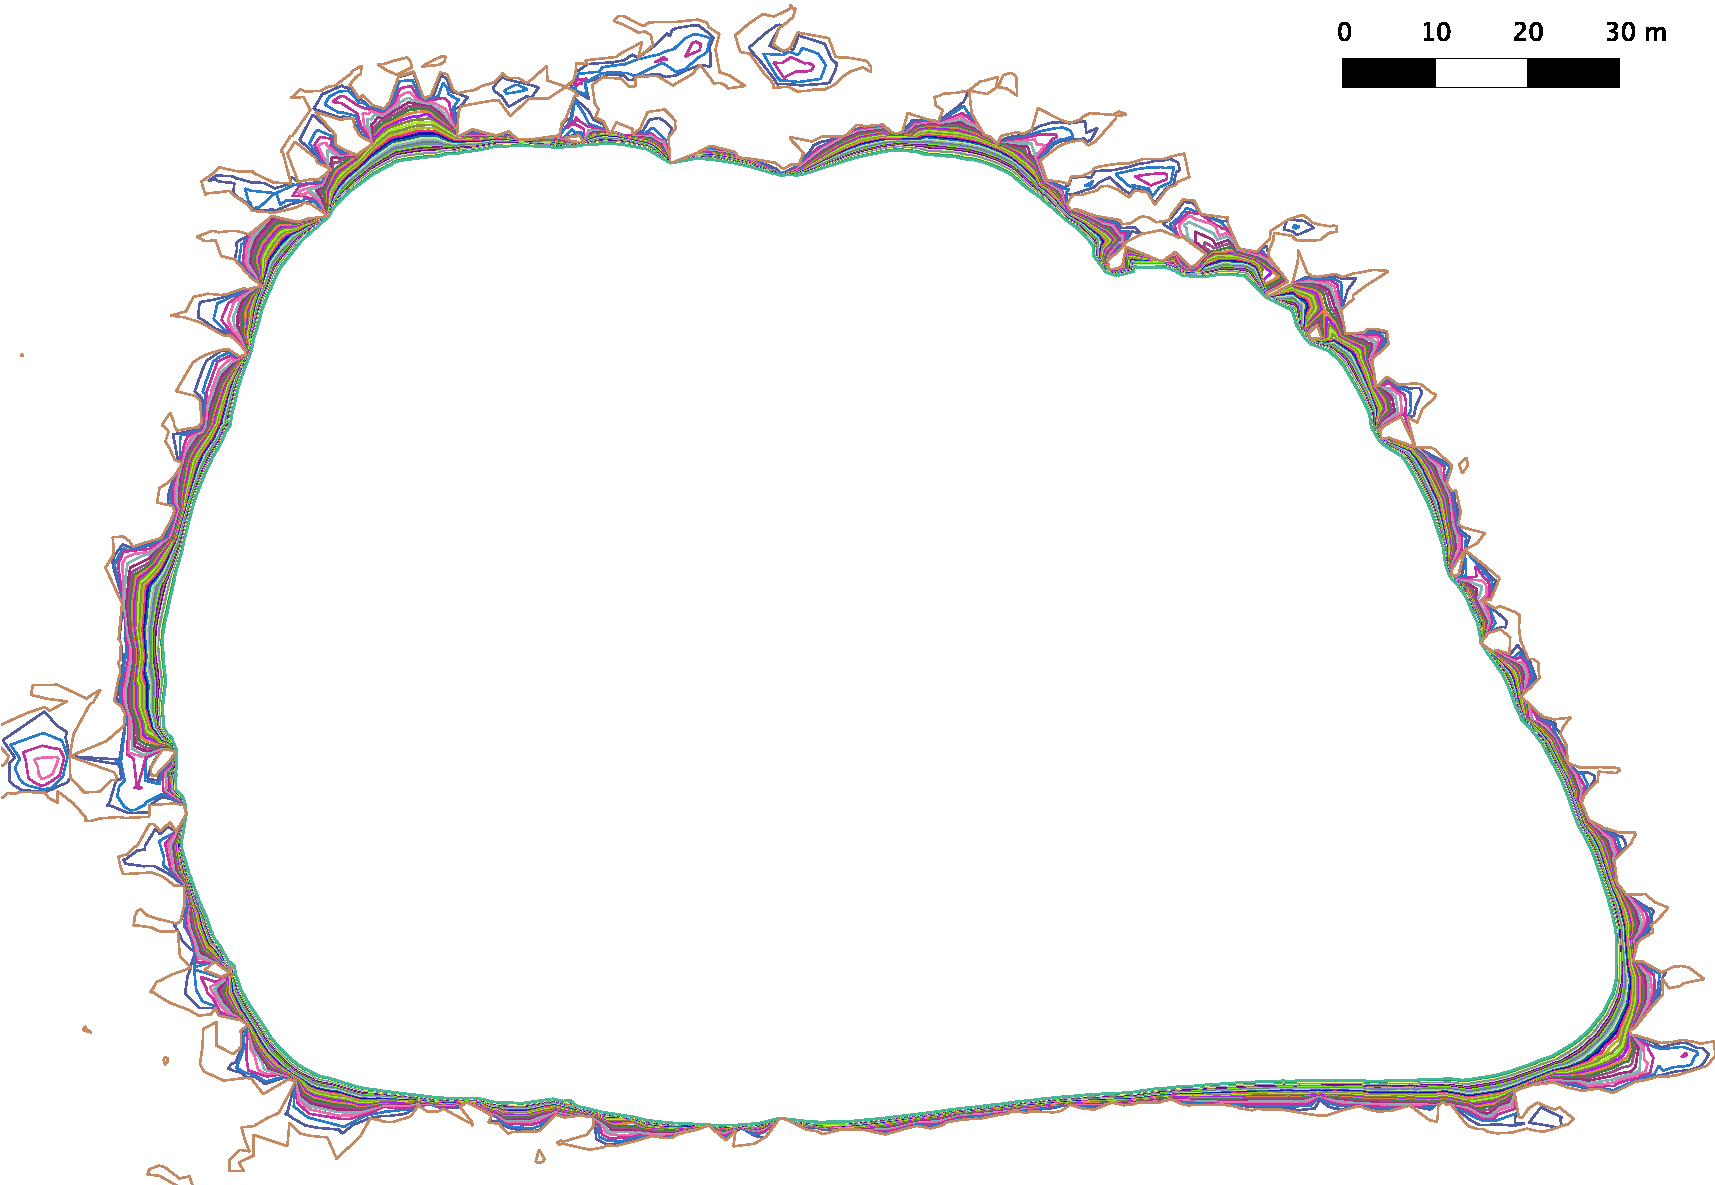
\includegraphics[width=0.95\linewidth]{figs/zl1845detailcontours0-30.pdf}
  \caption{From 0X smoothing (outer) to 30X smoothing (inner) for a given dataset.}
\label{fig:zl1845lineview}
\end{figure}
It is clear that the contour line moves towards the inner region, which is the deeper side of the contour, which is to be expected since the smoothing operator is safe per definition (and only lifts the surface upwards). 
What can also be seen is that the line is simplified (the details on the outer rim disappear, note however that the point count stays the same) and smoothed. 
% That is further supported by Figures~\ref{fig:zl1845lineview_o} and \ref{fig:zl1845lineview_s} that shows the point angularity before and after smoothing. It is evident that the number of points with a medium to high angularity are significantly reduced, which also corresponds to a smoother and more simplified contour line.


%%%%%%%%%%%%%%%%%%%%
%
\section{Notes \& comments}

The algorithm and the methodology of this chapter are (mostly) taken from \citet{Peters14}.

\citet{Zhang11} explains in detail how the generalisation of the content of a nautical chart is hindered by the four constraints.

% TODO : finish comments


%%%%%%%%%%%%%%%%%%%%
%
\section{Exercises}

\begin{enumerate}
  \item Explain why it is easier to respect the safety constraint using a TIN that has all the original MBES points as opposed to using a set of raw contours generated directly from that MBES dataset.
  \item Explain why simplification with Douglas-Peucker is not applicable in a bathymetric context. And give a concrete example.
  \item For a terrain ``on the land'', if Douglas-Peucker is used to simplify isocontours, what problems can be expected?
  \item The Laplace interpolation is used in the methodology presented, but would the natural neighbour interpolation method also be suitable?
\end{enumerate}